\documentclass[11pt]{article}
\usepackage[margin=1in]{geometry}
\usepackage{amsmath,amssymb}
\usepackage{booktabs}
\usepackage{xcolor}
\usepackage{graphicx}
\usepackage{parskip}        % no paragraph indent; separate paragraphs by vertical space
\usepackage{listings}
\usepackage{tikz}
\usetikzlibrary{positioning,arrows.meta,fit,backgrounds,calc,shapes.geometric}
\usepackage[colorlinks=true,linkcolor=blue,urlcolor=blue,citecolor=blue]{hyperref}

\definecolor{cset}{RGB}{31,119,180}
\definecolor{cfield}{RGB}{44,160,44}
\definecolor{cop}{RGB}{214,39,40}
\definecolor{cgray}{RGB}{120,120,120}

\lstdefinestyle{yaml}{
  basicstyle=\ttfamily\scriptsize,
  frame=single,
  backgroundcolor=\color{gray!7},
  columns=fullflexible,
  breaklines=true,
  keepspaces=true,
  showstringspaces=false,
  commentstyle=\color{cgray}\itshape,
  morecomment=[l]{\#},
}

\newcommand{\code}[1]{\texttt{#1}}

% GitHub repository as a clickable, line-breakable typewriter link: \ghrepo{org}{name}
\newcommand{\ghrepo}[2]{\href{https://github.com/#1/#2}{\texttt{#1/\allowbreak#2}}}

\title{\textbf{Plexus}\\[3pt]
\large A blueprint for differentiable tissue}
\author{Janelia Research Campus}
\date{\today}

\begin{document}
\maketitle

\begin{abstract}

A mechanism, in the account that philosophers of biology have converged on, is
\emph{entities and activities organized such that they are productive of regular
changes from start or set-up to finish or termination
conditions}.\footnote{Machamer, P., Darden, L.\ \& Craver, C.\,F.\ (2000). Thinking
about mechanisms. \emph{Philosophy of Science} 67:1--25, p.\,3.
\url{https://doi.org/10.1086/392759}. The hierarchical reading is developed in Craver,
C.\,F.\ (2007), \emph{Explaining the Brain}, Oxford University Press, and Craver \&
Darden (2013), \emph{In Search of Mechanisms}, University of Chicago Press.} We
introduce \emph{Plexus}, a language for writing a mechanism down in exactly those
terms, so that the description can be run, fitted to observations, and shown to be
missing an activity. A model is stated in two halves. \emph{What exists}: the
entities, of as many kinds as the hypothesis needs, the states they carry, the
relations between them and the levels that organize them. \emph{What happens}: the
activities acting on them. Neither half is subordinate to the other. An activity such
as adhesion has no meaning apart from what is adhering to what, and a model of a
tissue, its basement membrane and the surrounding matrix is informative precisely
because those remain distinct kinds of entity rather than being flattened into
variables of one universal object. Every activity therefore declares the entities it
acts upon, the states it requires, the relations it needs, and one or more numerical
implementations, while a hierarchy of levels keeps heterogeneous entities, fields and
relations organized rather than merged. Decomposition serves recomposition: the purpose
is to take existing models apart into reusable pieces and to build new biological
compositions from them, which in turn requires the language that specifies a model to
be separated from the interpreter that executes it. The Plexus research program has
three objectives. First, to define an algebra of activities over these organized
entities. Second, to decompose the existing corpus of simulation models into this
common language. Third, to construct differentiable implementations of these
activities so that mechanistic models can be directly inferred from biological data.

\end{abstract}

\section{Introduction}

Computational biology has produced a rich ecosystem of simulation frameworks.
Neural simulators model electrical activity, reaction--diffusion systems model
chemical transport, particle and continuum methods model mechanics, while
vertex, Cellular Potts and active-matter models describe multicellular tissues.
These frameworks remain however largely incompatible. Combining electrical
signalling, mechanics, metabolism and development often requires coupling multiple
specialized simulators whose underlying abstractions differ fundamentally. Each
simulator introduces its own representation of what a mechanism is, making models
difficult to compare, compose and extend. This fragmentation is not primarily a
numerical problem but a language problem.

Biology already has an account of what a mechanism is, even if it is rarely written
out. In the account of Machamer, Darden and Craver, a mechanism has two halves.
\emph{Entities} are the things: they have properties and stand in spatial relations to
one another. \emph{Activities} are what the things do: they are the producers of
change. And the two are \emph{organized}. Spatially, by location, shape and contact.
Temporally, by order, rate and duration. Hierarchically, because what the parts do at
one level constitutes what the whole does at the next. A mechanism starts from set-up
conditions and ends at termination conditions, and its description bottoms out in
activities that the field takes as fundamental. This is the account a cell biologist
uses tacitly whenever a paper ends with a summary figure: named parts, arrows between
them, boxes inside boxes. The paper has exact words for that figure. A \emph{mechanism
sketch} is a description with gaps, black boxes that no known activity yet fills. A
\emph{mechanism schema} is an abstract description whose placeholders can all be
filled with known parts and activities. A complete description exhibits
\emph{productive continuity without gaps} from set-up to termination conditions, and
the continuity lies in the arrows. The sketch cannot be run, cannot be fitted to data,
and cannot be shown to be missing an arrow.

Plexus takes that account literally. Instead of treating simulation frameworks as
fundamental, we treat entities and activities as the primary objects, and the
biological system itself as the thing to be decomposed. A system is decomposed not only
into activities but also into the entities those activities act upon. These entities
are heterogeneous, receptors, signalling proteins, cells, extracellular matrices,
tissues, fields, and they are organized across biological levels. Plexus makes that
organization explicit as a compositional hierarchy: each level carries its own
entities and states, activities act between entities within a level, and Aggregate and
Broadcast connect levels by mapping state upward and downward. Decomposition therefore
does not flatten biology into a single collection of variables; it preserves the
organization through which mechanisms at one level are composed with mechanisms at
another.

On the activity side, Plexus writes each one down independently of its numerical
implementation: adhesion, diffusion, division, chemotaxis, electrical propagation or
active stress. In a specification an activity is written as an \emph{operator}; the two
words name the same thing, and this paper uses the biological one except where it
names code. Entities and activities are the two halves of one decomposition, and
neither is primary. An activity is typed by the entities, states and relations it
requires, and a population of entities is inert until activities act on it.

The purpose of this decomposition is ultimately recomposition: to construct complete
mechanistic models from reusable entities and activities, rather than merely to
classify the mechanisms of existing simulators. Making such compositions executable
requires a strong structural choice. The language that specifies a biological model
must be separated from the code that interprets and executes it. The language declares
entities, states, relations, hierarchy and activities; the interpreter resolves that
description into concrete numerical implementations and schedules their execution. In
this perspective, biological modelling becomes analogous to compiler design: just as
modern compilers separate programming languages from their implementations through an
intermediate representation, Plexus separates biological mechanisms and their
organization from the numerical methods that realize them. The analogy is a consequence
of wanting free recomposition, not the premise it starts from. What the language
guarantees is that a hypothesis is well formed and complete. Whether it is
\emph{productive of} the change observed is what running it establishes.

This viewpoint defines a broader research program. First, Plexus seeks to construct an
algebra of activities whose elements can be composed into complex dynamical systems,
compared through their observable consequences, and expanded as new mechanisms are
discovered. Second, Plexus aims to extract this algebra from the existing corpus of
biological simulation models. Rather than viewing current frameworks as competing
simulators, we regard them as repositories of reusable entities and activities. By
decomposing these models into a common language, we seek to identify a compact
vocabulary capable of expressing a wide range of biological dynamics across scales.
Third, Plexus constructs differentiable counterparts of these compositions.
Differentiability allows mechanistic models to be fitted directly to biological data,
residuals to be interpreted mechanistically, and missing activities to be intuited.

Finally, because mechanisms are represented in a formal language rather than embedded
in simulator-specific code, they become amenable to automated reasoning. The explicit
separation between biological semantics and numerical implementations allows agentic
systems to operate directly on the language itself, composing, comparing and
optimizing mechanistic models without modifying simulator code. The search for
biological explanations therefore becomes a search over model structures rather than
simulator implementations.

%%%%%%%%%%%%%%%%%%%%%%%%%%%%%%%%%%%%%%%%%%%%%%%%%%%%%%%%%%%%%%%%%%%%%%%%%%%%%%%%
%%%%%%%%%%%%%%%%%%%%%%%%%%%%%%%%%%%%%%%%%%%%%%%%%%%%%%%%%%%%%%%%%%%%%%%%%%%%%%%%
\section{The language}

Plexus defines a typed language for expressing biological models independently of
their numerical realization. The language names \emph{what exists}: the
\emph{entities}, the \emph{states} they carry, the \emph{fields} they live in, the
\emph{relations} between them and the \emph{hierarchy} that organizes them. And it
names \emph{what happens}: the \emph{activities} that transform them. Biological
models are therefore represented as compositions of activities acting on organized
discrete and continuous biological objects rather than as simulator-specific
algorithms. The following subsections take these in turn: activities, entities,
states, fields, and the hierarchy that holds them.

%%%%%%%%%%%%%%%%%%%%%%%%%%%%%%%%%%%%%%%%%%%%%%%%%%%%%%%%%%%%%%%%%%%%%%%%%%%%%%%%
\subsection{Activities}

Activities are the fundamental objects of the language. An activity represents a
single biological mechanism, such as adhesion, chemotaxis, diffusion, electrical
propagation, active stress, metabolism, growth, or cell division. Every activity is
defined by a typed signature and one or more numerical implementations. The signature
specifies \emph{what} biological transformation is performed, whereas implementations
specify \emph{how} it is numerically realized. The signature specifies

\begin{itemize}
\item the entities the activity acts on,
\item the entities it changes,
\item the state variables consumed and produced,
\item the maps relating the participating entities.
\end{itemize}

Maps define the relations required by the mechanism. They determine, for example,
which particle belongs to which cell, which synapses connect which neurons, or how
cells relate to a continuous field. Plexus incorporates maps into the activity, making
activities typed morphisms between kinds of entities, so that the spatial organization
of the mechanism is declared with the activity rather than assumed by the code.

%%%%%%%%%%%%%%%%%%%%%%%%%%%%%%%%%%%%%%%%%%%%%%%%%%%%%%%%%%%%%%%%%%%%%%%%%%%%%%%%
\subsection{Entities}

Entities come in kinds: genes, proteins, cells, neurons, synapses, tissues, organs and
organisms. The entities of one kind form a set $S$, homogeneous in kind: its elements
share one state schema and one biological interpretation. In what follows a
\emph{kind} of entity and the set that holds it are the same object seen from biology
and from mathematics.

Kinds organize into hierarchies reflecting biological organization, but a level of
that hierarchy is \emph{not} a single kind, and this is the point at which a familiar
simplification has to be resisted. Writing the hierarchy as a chain
$S_0 \to S_1 \to S_2 \to S_3$, molecules, then cells, then tissues, then organism,
suggests one biological category per level. Biology is not so uniform. A cell contains
receptors, signalling proteins, cytoskeletal elements and, in a mechanical model,
material points; a tissue contains cells, a basement membrane and an extracellular
matrix. Each of those is a distinct kind with its own state and its own activities,
and all of them share a parent. A level is therefore a heterogeneous collection

\[
L_k = \{\, S_k^1, S_k^2, \ldots,\; F_k^1, F_k^2, \ldots,\; R_k^1, R_k^2, \ldots \,\},
\]

of kinds $S_k^i$, fields $F_k^j$ bound to that level, and relations $R_k^l$ among
them. The hierarchy organizes these objects; it does not define them by a single
molecule/cell/tissue label. Each level is expressed in the same language, allowing
intracellular signalling, multicellular mechanics, developmental processes and
organ-level physiology to be described without translation between formalisms.

%%%%%%%%%%%%%%%%%%%%%%%%%%%%%%%%%%%%%%%%%%%%%%%%%%%%%%%%%%%%%%%%%%%%%%%%%%%%%%%%
\subsection{States}

Every entity carries a state describing its current biological condition. While
entities define \emph{what} exists, states define \emph{what each entity carries}.
The state schema is specific to each kind. A protein may carry position, binding state
and the load it bears; a material point position, velocity and deformation gradient; a
neuron membrane voltage and calcium; a cell polarity, stiffness and gene-expression
levels; a synapse conductance and plastic weight. Activities transform states. They
consume selected state variables and produce updates to others, while leaving the
underlying entities unchanged.

%%%%%%%%%%%%%%%%%%%%%%%%%%%%%%%%%%%%%%%%%%%%%%%%%%%%%%%%%%%%%%%%%%%%%%%%%%%%%%%%
\subsection{Fields}

Fields represent continuous quantities defined over space rather than over discrete
entities. Examples include morphogen concentrations, pressure, extracellular
signalling molecules, electric potentials, and material properties. Fields complement
entities. While entities are the discrete parts, fields describe the continuous
environment, the microenvironment, in which these parts evolve. Activities couple
entities and fields through explicit maps relating discrete entities to continuous
spatial representations.

%%%%%%%%%%%%%%%%%%%%%%%%%%%%%%%%%%%%%%%%%%%%%%%%%%%%%%%%%%%%%%%%%%%%%%%%%%%%%%%%
\subsection{Hierarchy}\label{sec:hierarchy}

Containment is declared, not implied. Entities of one kind may be contained in
entities of another, proteins in a cell, cells in a tissue, tissues in an organism,
through an explicit map $\pi$ from children to parent. A parent may contain several
distinct kinds at once: the same cell can hold receptors, signalling proteins,
cytoskeletal elements and material points, each remaining a distinct object with its
own state and its own activities while sharing that parent. Every level carries its
own state, its own activities and its own rate, so no level is reduced to a parameter
of the level above it.

\begin{figure}[h]
\centering
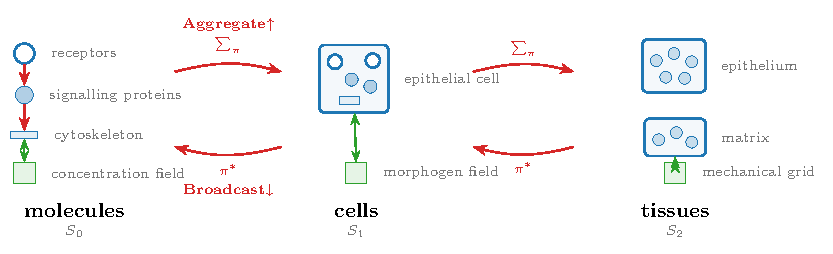
\includegraphics[width=0.80\textwidth]{fig_hier.pdf}
\caption{The hierarchy. Each level holds several \emph{distinct} kinds of entities
(blue) and may carry its own fields (green); activities (red) act between entities
within a level, and exactly two families cross a level: Aggregate, $\sum_\pi$, and
Broadcast, $\pi^{*}$.}
\label{fig:hier}
\end{figure}

Activities act within a level or across levels. Within a cell, activities may couple
receptors to signalling proteins to cytoskeleton. Across the containment map, exactly
two families apply. \textbf{Aggregate} is integration: it builds parent state from
children, a cell position from its material points, a neuron input from its synapses.
\textbf{Broadcast} is top-down control: it propagates parent state to children, a
material property to every point a cell owns, or a constraint imposed by the parent.
Formally,

\[
L_k \;\xrightarrow{\ \text{Aggregate}\ }\; L_{k+1},
\qquad
L_{k+1} \;\xrightarrow{\ \text{Broadcast}\ }\; L_k .
\]

$\pi$ is a \emph{function}, and that is load-bearing rather than a formality. A
function partitions the children into fibres $\pi^{-1}(p)$, and it is that partition
which makes Aggregate well defined: every child is counted exactly once, so the sum
conserves. Broadcast is its adjoint. A many-to-many relation would admit neither.
Aggregating over one needs weights to avoid counting a shared child several times, and
no weighting is canonical.

\paragraph{Many-to-many relations need no new primitive.} Much biological structure
is not a function. A vertex of an epithelial mesh belongs to three cells at once, so
vertex $\to$ cell cannot be written as $\pi$. This does not call for a second kind of
hierarchy: a relation $R \subseteq A \times B$ \emph{is} a kind of entity $R$ together
with two functions $R \to A$ and $R \to B$, so a relation is represented by giving it
the status of entities, and both of its legs are ordinary containment maps. Synapses
with \code{pre} and \code{post} are exactly this, a many-to-many relation between
neurons carried as a population of pairs, and so is the half-edge table of a mesh,
whose every half-edge has exactly one source vertex and exactly one face. Aggregating
half-edge quantities onto faces (a cell's area, its perimeter) is $\sum_\pi$ along the
second leg, and reading vertex positions at half-edges is $\pi^{*}$ along the first.
The two cross-level families are therefore sufficient for structure that is not
itself hierarchical, provided the relation is given the status of entities.

Fields are level-specific in the same way. Exchange couples entities to a field at
their own level, so a molecular concentration field, a cellular morphogen field and a
tissue-scale mechanical grid coexist as distinct objects rather than being merged into
one grid.

The consequence is that molecules, cells and tissues are not a pipeline of separate
simulators handing results to one another. They are one compositional graph: several
kinds may coexist inside each parent, activities connect them locally, and Aggregate
and Broadcast connect the levels. The same families are reused throughout, so adding a
biological scale adds no machinery to the engine.

%%%%%%%%%%%%%%%%%%%%%%%%%%%%%%%%%%%%%%%%%%%%%%%%%%%%%%%%%%%%%%%%%%%%%%%%%%%%%%%%
%%%%%%%%%%%%%%%%%%%%%%%%%%%%%%%%%%%%%%%%%%%%%%%%%%%%%%%%%%%%%%%%%%%%%%%%%%%%%%%%
\section{The algebra of activities}

The language introduced in the previous section defines the objects manipulated by
Plexus. We now define the elementary families of activities from which biological
models are constructed. The central hypothesis of Plexus is that a large fraction of
existing biological simulation models can be expressed as compositions of a small
number of elementary families. Rather than introducing a new activity for every
biological phenomenon, Plexus identifies a compact algebra that can be reused across
mechanics, signalling, metabolism, development and physiology.

The proposed algebra consists of eight elementary families (Fig.~\ref{fig:ops}), each
named here first in a biologist's words:

\begin{itemize}
\item \textbf{Lateral}: what neighbours do to each other among entities of one kind.
\item \textbf{Aggregate}: integration, a whole reading its parts, many-to-one across levels.
\item \textbf{Broadcast}: top-down control, a whole imposing on its parts, one-to-many across levels.
\item \textbf{Exchange}: traffic between entities and their microenvironment, the fields.
\item \textbf{Rewire}: remodelling, a change of the relations between entities.
\item \textbf{Divide}: proliferation, the creation of entities.
\item \textbf{Die}: apoptosis and extrusion, the removal of entities.
\item \textbf{Seed}: the set-up conditions, the establishment of the initial state.
\end{itemize}

The first four families transform biological state while preserving the underlying
organization. Rewire modifies the relations, whereas Divide and Die modify the
entities themselves. Seed writes the state a model starts from. Together they form the
elementary computational vocabulary of Plexus.

Seed is separated from Divide and Die, with which it shares a mechanism since all three
write state directly rather than returning a delta, because it differs in \emph{when}.
Divide and Die act throughout a trajectory; Seed acts only at its opening. Treating
that distinction as a naming convention rather than a kind has a concrete cost. In an
automated model-search campaign on a growing epithelial vesicle, an initial condition
for a reaction--diffusion field was re-applied on every timestep rather than once,
which converts it from an initial condition into a moving boundary condition and
silently overwrites the state of any activity writing to the same channel. Both
spellings were legal specifications and nothing in the language could distinguish
them; the resulting runs reported a mechanism as refuted eight times across thirteen
rounds when the activity under test had in fact never reached the state. Because Seed
is a kind, the runtime imposes its window, and a per-timestep initial condition is not
expressible.

\begin{figure}[h]
\centering
\resizebox{\textwidth}{!}{%
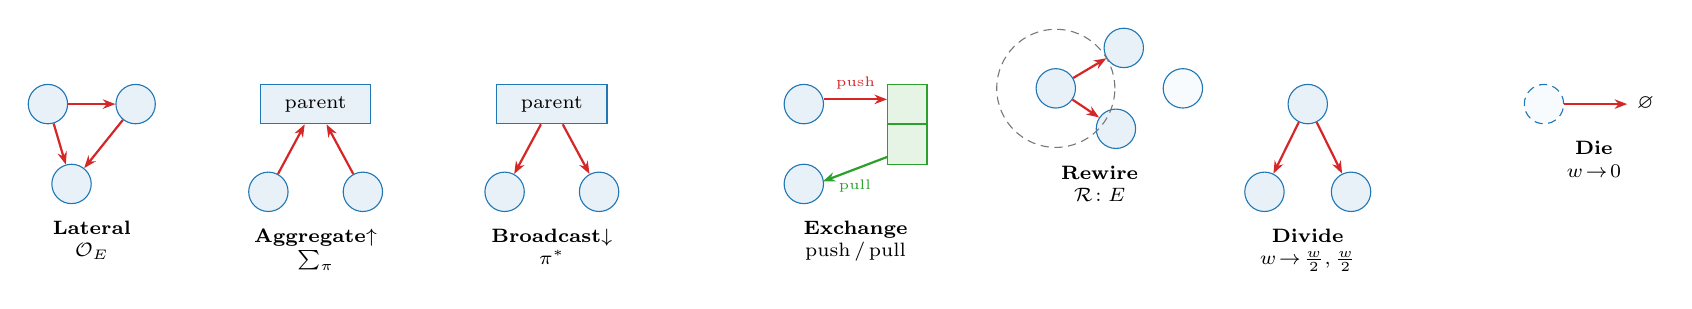
\begin{tikzpicture}[
  font=\scriptsize,
  n/.style={circle,draw=cset,fill=cset!10,minimum size=5mm,inner sep=0},
  p/.style={rectangle,draw=cset,fill=cset!10,minimum width=14mm,minimum height=5mm},
  g/.style={rectangle,draw=cfield,fill=cfield!12,minimum width=5mm,minimum height=5mm},
  a/.style={-{Stealth[length=1.6mm]},cop,thick},
]
\begin{scope}[local bounding box=L]
  \node[n] (a1){}; \node[n,right=6mm of a1](a2){}; \node[n,below=5mm of a1,xshift=3mm](a3){};
  \draw[a] (a1)--(a2); \draw[a] (a1)--(a3); \draw[a] (a2)--(a3);
\end{scope}
\node[below=1mm of L,align=center]{\textbf{Lateral}\\$\mathcal{O}_E$};
\begin{scope}[shift={(34mm,0)},local bounding box=A]
  \node[p] (par){parent};
  \node[n,below=6mm of par,xshift=-6mm](c1){}; \node[n,below=6mm of par,xshift=6mm](c2){};
  \draw[a] (c1)--(par); \draw[a] (c2)--(par);
\end{scope}
\node[below=1mm of A,align=center]{\textbf{Aggregate}$\uparrow$\\$\sum_\pi$};
\begin{scope}[shift={(64mm,0)},local bounding box=B]
  \node[p] (par2){parent};
  \node[n,below=6mm of par2,xshift=-6mm](d1){}; \node[n,below=6mm of par2,xshift=6mm](d2){};
  \draw[a] (par2)--(d1); \draw[a] (par2)--(d2);
\end{scope}
\node[below=1mm of B,align=center]{\textbf{Broadcast}$\downarrow$\\$\pi^*$};
\begin{scope}[shift={(96mm,0)},local bounding box=E]
  \node[n] (o1){}; \node[n,below=5mm of o1](o2){};
  \node[g,right=8mm of o1](g1){}; \node[g,below=0mm of g1](g2){};
  \draw[a,transform canvas={yshift=0.6mm}] (o1)-- node[above,font=\tiny]{push}(g1);
  \draw[a,cfield,transform canvas={yshift=-0.6mm}] (g2)-- node[below,font=\tiny]{pull}(o2);
\end{scope}
\node[below=1mm of E,align=center]{\textbf{Exchange}\\push\,/\,pull};
% --- structure operators (rewire the edges E, change the node set |S|) ---
\begin{scope}[shift={(128mm,2mm)},local bounding box=RW]
  \node[n] (rc){};
  \node[n,above right=1.5mm and 5mm of rc](rn1){};
  \node[n,below right=1.5mm and 4mm of rc](rn2){};
  \node[n,right=11mm of rc,fill=cset!3](rn3){};
  \draw[densely dashed,cgray] (rc) circle (7.5mm);
  \draw[a] (rc)--(rn1); \draw[a] (rc)--(rn2);
\end{scope}
\node[below=1mm of RW,align=center]{\textbf{Rewire}\\$\mathcal{R}\!:E$};
\begin{scope}[shift={(160mm,0)},local bounding box=DV]
  \node[n] (m){};
  \node[n,below=6mm of m,xshift=-5.5mm](g3){}; \node[n,below=6mm of m,xshift=5.5mm](g4){};
  \draw[a] (m)--(g3); \draw[a] (m)--(g4);
\end{scope}
\node[below=1mm of DV,align=center]{\textbf{Divide}\\$w\!\to\!\tfrac{w}{2},\tfrac{w}{2}$};
\begin{scope}[shift={(190mm,0)},local bounding box=DE]
  \node[n,densely dashed,fill=cset!3] (z){};
  \node[right=8mm of z] (nul) {$\varnothing$};
  \draw[a] (z)--(nul);
\end{scope}
\node[below=1mm of DE,align=center]{\textbf{Die}\\$w\!\to\!0$};
\end{tikzpicture}}
\caption{
The elementary algebra of activities of Plexus. Lateral, Aggregate, Broadcast and
Exchange transform biological state. Rewire modifies relations, whereas Divide and
Die modify the entities. Complex biological models are obtained by composing these
elementary families.
}
\label{fig:ops}
\end{figure}

\paragraph{Lateral.}
Lateral activities are what entities of one kind do to one another. Typical examples
include mechanical forces between proteins, adhesion and tension between neighbouring
cells, juxtacrine signalling, electrical communication between neurons, or biochemical
interactions within a metabolic network.

\paragraph{Aggregate.}
Aggregate activities are integration: a whole reads its parts, propagating information
from many entities to a higher level of organization. Examples include computing
cellular properties from their constituent proteins or accumulating synaptic currents
acting on a neuron. This is the upward direction of causation, the one usually called
emergence.

\paragraph{Broadcast.}
Broadcast activities are top-down control: a whole imposes on its parts, propagating
information from higher organizational levels toward their constituents. Aggregate and
Broadcast therefore define the upward and downward flow across biological levels.

\paragraph{Exchange.}
Exchange activities couple discrete entities with continuous fields: a cell's traffic
with its microenvironment. Typical examples include secretion, sensing, transport,
uptake, or particle--grid transfer.

\paragraph{Rewire.}
Rewire activities are remodelling. They modify the relations between entities without
changing the entities themselves, updating neighbour graphs, contact networks,
developmental connectivity or other interaction structures, and so determining which
entities participate in subsequent activities.

\paragraph{Divide and Die.}
Living systems continuously modify their own composition; this is turnover. Divide
creates new entities, whereas Die removes existing ones. These activities modify the
biological organization itself rather than only its state, and they are what makes a
tissue different from any inert material.

%%%%%%%%%%%%%%%%%%%%%%%%%%%%%%%%%%%%%%%%%%%%%%%%%%%%%%%%%%%%%%%%%%%%%%%%%%%%%%%%
\section{Composition}

A biological model is built by composition, and composition happens in four
distinct ways. Each answers a different question, and a model is complete only
when all four are answered.

\begin{enumerate}
\item \textbf{Entities compose into structures.} The kinds of entities, the states
they carry and the relations declared between them form the objects a model is about:
a membrane is a population of faces with an incidence relation, a connectome is a
population of neurons with an edge population over it, a tissue is a population of
cells with a containment map to its molecules. This composition is structural and is
fixed by the specification before any dynamics run.

\item \textbf{Activities compose within a level.} Several activities may act on the
same entities, each contributing its own increment: adhesion and active stress on one
population of cells, diffusion and reaction on one chemical field. Because activities
are typed by what they read and write rather than by the simulator they came from,
mechanisms from different modelling traditions may act side by side on the same
entities.

\item \textbf{Levels compose through Aggregate and Broadcast.} A mechanism
written at one level reaches another only through the containment map of
Section~\ref{sec:hierarchy}, $L_k \to L_{k+1}$ upward and $L_{k+1} \to L_k$
downward. This is what allows a molecular mechanism and a tissue-scale mechanism
to belong to one model without either being rewritten in the other's terms.

\item \textbf{Activities compose in time.} The three compositions above say what
acts on what; the \emph{schedule} says in which order and how often. This is the
temporal organization of the mechanism: its order, rate and duration.
\end{enumerate}

The first three are the subject of the preceding sections. The remainder of this
section formalizes the fourth.

Rather than embedding all mechanisms within a monolithic simulator, Plexus
represents a model as an ordered sequence of activities. This sequence, called the
\emph{schedule}, specifies both the order and the frequency with which activities are
evaluated. Formally, one simulation step is the composition

\[
\Phi
=
\mathcal O_n
\circ
\cdots
\circ
\mathcal O_1,
\]

whose repeated application generates the system dynamics

\[
x_{t+1}
=
\Phi(x_t).
\]

The schedule therefore describes the temporal organization of biological
mechanisms. Different activities may evolve on different time scales. Mechanical
interactions may be evaluated every simulation step, whereas diffusion, growth or cell
division may occur less frequently. A biological model therefore becomes a multi-rate
composition of biological mechanisms rather than a monolithic numerical solver.

Activities are pure transformations. Rather than modifying biological state directly,
every activity returns its contribution to the system evolution. If activity
$\mathcal O_i$ produces the increment $\Delta_i$, the complete update is obtained by

\[
\Delta
=
\sum_i
\Delta_i,
\]

before being passed to the numerical implementation. This formulation has two
important consequences. First, biological mechanisms remain independent and
composable: introducing a new mechanism simply requires adding a new activity to the
schedule. Second, the language remains independent of its numerical realization. The
schedule specifies the biological model, whereas the numerical implementation
specifies how that model is evaluated.

%%%%%%%%%%%%%%%%%%%%%%%%%%%%%%%%%%%%%%%%%%%%%%%%%%%%%%%%%%%%%%%%%%%%%%%%%%%%%%%%
\section{Bottoming out: numerical implementations}

Every mechanistic description stops somewhere. It bottoms out in activities the field
is content to take as given. In Plexus that floor is the numerical implementation. The
algebra of activities defines the biological semantics of a model independently of its
numerical realization. Every activity may admit multiple implementations satisfying the
same typed signature. These implementations differ in numerical realization while
preserving identical biological semantics. Selecting an implementation is therefore a
numerical decision rather than a biological one.

This abstraction naturally accommodates a broad range of computational methods.
Mechanical activities may be implemented using Material Point Methods, finite
elements, vertex models, phase-field methods, Cellular Potts models or
optimal-transport formulations. Signalling activities may employ Hodgkin--Huxley
equations, graph neural networks or Neural ODEs. Likewise, field activities may use
finite differences, finite elements, neural implicit representations or spectral
methods. These implementations coexist within the same language because they satisfy
identical contracts.

Different implementations may also employ different numerical integration schemes.
Depending on the activity, implementations may evolve first-order states such as
concentrations or membrane voltages, second-order states such as mechanical
accelerations, or rely on explicit, implicit or adaptive solvers. These choices affect
computational efficiency and numerical accuracy but not the biological interpretation
of the model.

This distinction fundamentally changes how biological simulations are compared.
Traditional frameworks compare complete simulators, intertwining biological
mechanisms with numerical algorithms. Plexus instead separates these two questions.
Biological models are compared through the activities they compose, whereas numerical
methods are compared through the implementations realizing those activities.

Because biological mechanisms are represented in a formal language rather than
embedded in simulator-specific code, they become amenable to automated reasoning. The
explicit separation between biological semantics and numerical implementations allows
agentic systems to operate directly on the language itself, composing, comparing and
optimizing mechanistic models without modifying simulator code. The search for
biological explanations therefore becomes a search over model structures rather than
simulator implementations.

%%%%%%%%%%%%%%%%%%%%%%%%%%%%%%%%%%%%%%%%%%%%%%%%%%%%%%%%%%%%%%%%%%%%%%%%%%%%%%%%
\section{Mechanistic inverse modelling}

One of the primary motivations for introducing a formal language of biological
mechanisms is to identify mechanistic models directly from experimental observations.
Rather than calibrating simulations manually, the objective is to infer the
parameters, spatial organization and constitutive laws governing biological systems
from imaging data.

Plexus makes this possible by associating every activity with one or more
differentiable implementations satisfying the same typed signature. Differentiability
therefore becomes a property of the language rather than of a particular simulator.
Regardless of the numerical backend, gradients propagate through compositions of
explicit activities rather than through monolithic simulation code.

This distinction fundamentally changes the role of inverse modelling. Traditional
approaches assume that the underlying mechanism is already correct and seek the
parameter values that best reproduce the observations. Such parameter optimization is
effective when the forward model is complete, but it becomes misleading when important
activities are absent. Optimizing existing parameters may improve the fit while merely
compensating for missing activities.

In Plexus, parameters remain attached to explicit activities rather than to opaque
numerical models. Mechanical properties belong to mechanical activities, reaction
rates to biochemical activities, conductances to signalling activities, and spatial
fields to the mechanisms generating them. Parameter estimation therefore preserves the
mechanistic interpretation of the model.

Residuals likewise acquire a mechanistic interpretation. A persistent mismatch between
simulation and experiment no longer indicates only poor parameter values; it may also
indicate that the current composition of activities is unable to explain the
observations. In the terms of Machamer, Darden and Craver, a residual that will not go
away is the mark of a sketch: a black box where an activity belongs. Differentiability
thus provides more than efficient optimization: it enables quantitative comparison
between competing mechanistic models while preserving their explicit biological
structure.

Crucially, because the composition is differentiable end to end, the objective need not
span the entire system: a loss may be \emph{local} in both space and time. It can be
evaluated on a chosen \emph{subset of entities}, a region of interest such as the
extrusion front where activated and quiescent cells meet, over a \emph{short rollout}
of a few tens of steps, rather than on every cell across the whole trajectory.
Gradients still propagate through the shared composition, so a \emph{local} objective
fine-tunes precisely the mechanism responsible for a local behaviour, the shape of a
growth front, the sharpness of a domain boundary, the timing of a rearrangement,
without the averaging-out of a global fit and, decisively, without the prohibitive cost
of differentiating a long, whole-system rollout. This last point is what makes the
approach practical at all: a loss spanning every cell over hundreds of frames unrolls,
under reverse-mode differentiation, into a backpropagation graph whose memory and
compute scale as cells~$\times$~steps and quickly become intractable, whereas a loss
confined to a few entities over a short window keeps that gradient graph small.
\emph{Locality} is therefore the enabling property of differentiable refinement on
large, long-lived tissues: the mechanism is global and shared, but the \emph{evidence}
constraining any single activity is usually confined to a small, transient region, and
the loss should be placed exactly there.

%%%%%%%%%%%%%%%%%%%%%%%%%%%%%%%%%%%%%%%%%%%%%%%%%%%%%%%%%%%%%%%%%%%%%%%%%%%%%%%%
\section{Agentic mechanistic discovery}

\begin{quote}
\emph{``What I cannot create, I do not understand.''} \\
\emph{``Know how to solve every problem that has been solved.''}

\hfill Richard P.\ Feynman\footnote{Found written on Feynman's blackboard at
Caltech at his death in February 1988. Never published in a paper or lecture, it
survives as a bare aphorism; the second line stood directly beneath the first on the
same board. Photographs of the blackboard are widely reproduced.}
\end{quote}

Feynman's two lines frame this section. A biological mechanism is understood only when
an agent can \emph{create} it, assembling it from activities until it reproduces the
observations, and new discovery begins only once the agent can already re-derive every
model that has been solved. The three loops below make this operational, moving from
reconstructing what is already known toward constructing the mechanisms that existing
models cannot yet express.

The explicit representation of biological mechanisms transforms scientific discovery
from a parameter optimization problem into a language exploration problem. Because
activities are declared rather than embedded in simulator-specific code, they become
directly accessible to agentic systems.

Plexus proposes a three-loop strategy for mechanistic discovery. Each loop operates at
a different level of abstraction, progressively moving from existing models toward new
biological knowledge.

\paragraph{Loop I: Understanding.}

The first loop takes an existing model, a paper and its repository, and decomposes it
into Plexus activities, entities, states and fields, so the mechanisms it implements
become explicit. That decomposition is necessary, but it is only the \emph{entry}: it
makes the model's \emph{levers} explicit without yet explaining them. Understanding is
earned afterwards, by \emph{interrogating} the decomposition as a causal system,
learning what each activity and parameter does on its own and, the harder part, what it
does in combination, since mixtures rarely surrender their causal structure to
inspection. The driving force is therefore not translation but a \emph{hypothesis
$\to$ validate/falsify} cycle run on the decomposed model: each step states a
falsifiable claim about a lever, tests it against a dedicated metric, and accumulates
the causal map that results. A useful operating point is a rough \textbf{70/30 balance
of validation to falsification}. Pure validation only ever confirms hypotheses one
already believes (trivial, near-zero information), while pure falsification only ever
probes the improbable (which mostly breaks as expected and never consolidates a working
map), so most tests should confirm plausible levers while a deliberate minority attacks
the current understanding, where a surprise is most informative. The loop's product is
a causal lever-map of the model, what each mechanism buys and how mechanisms combine,
which is what makes the activities genuinely \emph{reusable} rather than merely
catalogued, and what later tells Loop~III which lever the model \emph{lacks}.

\paragraph{Loop II: Fitting.}

The second loop estimates the parameters, spatial fields and set-up conditions of the
resulting mechanistic model by fitting it directly to experimental observations.
Because every activity admits a differentiable implementation, optimization preserves
an explicit correspondence between parameters and biological mechanisms.

\paragraph{Loop III: Discovery.}

The third loop analyses the residual remaining after optimization. Persistent
discrepancies are interpreted as evidence that the current composition of activities
is incomplete rather than simply poorly parameterized. Turning Loop~I's
hypothesis-driven validate/falsify cycle outward, from the levers the model \emph{has}
to the ones it \emph{lacks}, the agent proposes candidate activities, compares
competing mechanistic hypotheses, and extends the algebra whenever existing mechanisms
fail to explain the observations. It turns a sketch into a schema, one filled box at a
time.

Together, these three loops transform simulation, inverse modelling and hypothesis
generation into successive stages of a single scientific workflow. The language itself
becomes the object of discovery: new biological knowledge is represented by extending
the algebra of activities rather than merely adjusting parameter values.

\paragraph{Orchestration: loop agents and a master controller.}
The three loops are realized as autonomous agents coordinated by a \emph{master}: each
performs one kind of work, Understanding, Fitting, or Discovery, and communicates only
through typed artifacts on a shared blackboard (the mechanistic model, the success metrics
with current values, the residual, and a queue of falsifiable hypotheses). The master never
performs the loops' work; it is a state machine whose guards are the metrics. It advances a
stage when its metric is met, invokes Discovery when a residual persists, and re-invokes Fitting
once a new activity is admitted. Beyond scheduling it carries a few responsibilities: it
\emph{authors} the success metrics, so ``goal achieved'' is a falsifiable test rather than a
visual impression; it \emph{grounds} hypotheses in the reference literature and code before
Discovery proposes; it gates every proposal on \emph{compliance} (a well-typed Plexus
contract, not a simulator-specific patch) and \emph{consistency} (an active search for
violated invariants, determinism, conservation, agreement between overlapping runs,
that separates ``the model is incomplete'' from ``the measurement is wrong''); and it holds
each stage open until settled, refusing the ``good enough to move on'' shortcut.

\paragraph{The master reproduces a modeller's discipline.}
These responsibilities are not invented for the machine; they formalise how a careful
modeller works, distilled from a prototype that deciphers the \texttt{tyssue} epithelial
vertex model into Plexus activities.\footnote{Reported separately as a living document of
dated field notes: it reconstructs the model as mechanism-named contracts and works each
morphogenesis stage by the method below.} Four disciplines recur.
\begin{itemize}
\item \textbf{Verify the instrument before trusting the measurement.} The sharpest,
most-repeated lesson: a ``$97\%$ hollow'' shell that was a recording-stride \emph{misalignment}
(vertex positions paired with another frame's connectivity, caught by a determinism
contradiction, a long run diverging from its own shorter prefix), and a false
``$0$ invalid faces'' that passed self-intersecting bow-tie polygons because the guard checked
area $> 0$, not a simple embedded tiling. An agent that skips this gate elaborates activities
to explain an artefact.
\item \textbf{Small, falsifiable, metric-gated steps: one factor at a time, cheap-first.}
Loop~I's validate/falsify cadence, enforced across every stage: isolating proliferation rate,
division timing and volume stiffness is what homogenised the tissue; a blind sweep would not
attribute the win.
\item \textbf{Perfecting.} A satisfied metric is not qualitative fidelity: the
triangular-versus-round-cells gap became a newly authored metric (shape index, sliver
fraction) and a target to close.
\item \textbf{A persistent, revisable master memory.} A log of hypotheses validated and
overturned, grounding reads from the reference literature, and the atlas of activities, so the
search accumulates knowledge instead of re-deriving it each round.
\end{itemize}

\paragraph{What the loop cannot yet supply, and the agents that must.}
A prototype run with a human in the loop makes the division of labour precise, and honest
about its frontier: the worker agents are strong at execution, breadth and bookkeeping, but
four contributions came reliably from the human and name what the scheme must still
internalise.
\begin{itemize}
\item \textbf{Goal custody.} The single most valuable intervention. A worker elaborates
whatever it is touching and cannot catch its own drift (``I thought we were starting tubing
from 2000 cells''); the master's objective must be held \emph{separately} from the workers'.
\item \textbf{Temporal perception.} A genuinely structural gap: an agent reads a static
strip but cannot \emph{watch a movie}, yet the decisive evidence was in the time course
(a pattern that forms only at 12\,s; a spot that decays then reforms; tip cells that balloon
at 2\,s). A dynamics-watching critic is a required agent, not a convenience.
\item \textbf{Domain priors and taste.} Reading the activator gradient off Okuda's figure;
naming amplification feedback before finding it is Gierer--Meinhardt.
\item \textbf{Literature grounding.} ``which reaction--diffusion regime does Okuda use?''
$\to$ the GM unlock.
\end{itemize}
A faithful multi-agent scheme is therefore not one master and identical workers but a small
division of labour, a goal-custody supervisor, a dynamics-watching critic, and a
literature-grounding reader, around the disciplined loops above.


%%%%%%%%%%%%%%%%%%%%%%%%%%%%%%%%%%%%%%%%%%%%%%%%%%%%%%%%%%%%%%%%%%%%%%%%%%%%%%%%
%%%%%%%%%%%%%%%%%%%%%%%%%%%%%%%%%%%%%%%%%%%%%%%%%%%%%%%%%%%%%%%%%%%%%%%%%%%%%%%%
\appendix

\section{Reference implementation}
\label{app:reference}

In the code an activity is an \code{Operator} class and a kind of entity is a \code{Level} holding a set; the appendices use the code's names.

The main text defines Plexus as a formal language for expressing biological
mechanisms. This appendix describes the reference implementation of that
language. The implementation follows the abstractions introduced in the paper
without introducing additional biological concepts. Its purpose is simply to
execute models written in the Plexus language.

The implementation distinguishes two levels. The \emph{language} defines the
biological semantics through operators, sets, states and fields. The
\emph{runtime} provides concrete software classes implementing these concepts.

\begin{center}
\renewcommand{\arraystretch}{1.2}
\begin{tabular}{ll}
\toprule
\textbf{Language} & \textbf{Reference implementation}\\
\midrule
Operator (contract) & \code{OperatorContract}\\
Implementation & an \code{Operator} subclass, registered under a contract\\
Set & \code{Level}\\
State & typed tensors stored by a \code{Level} (sliced by its \code{state\_schema})\\
Map & an index buffer on a \code{Level} (\code{parent}, \code{pre}, \code{post})\\
Field & \code{Field}\\
Biological model & \code{Hierarchy}\\
Registry & \code{@register\_operator} / \code{@register\_entity} / \code{@register\_field}\\
\bottomrule
\end{tabular}
\end{center}

Maps are not a separate runtime object. Consistently with the operator-centric
view of the main text, a map is an index buffer carried by a \code{Level}
(\code{parent}/\code{parent\_name} for containment, \code{pre}/\code{post} for
incidence) and \emph{named} by the operators that traverse it in their typed
signature --- so the runtime realizes four primitives (operators, sets, states,
fields), with maps folded into the operator.

%%%%%%%%%%%%%%%%%%%%%%%%%%%%%%%%%%%%%%%%%%%%%%%%%%%%%%%%%%%%%%%%%%%%%%%%%%%%%%%%

\subsection{Hierarchy}

The \code{Hierarchy} represents one executable biological model. It is the
runtime container responsible for assembling the language primitives into a
simulation.

A Hierarchy stores

\begin{itemize}
\item the collection of biological Levels,
\item the continuous Fields,
\item the instantiated Operators,
\item the execution Schedule,
\item backend-specific runtime data.
\end{itemize}

The Hierarchy therefore corresponds to one complete biological model expressed
in the Plexus language.

%%%%%%%%%%%%%%%%%%%%%%%%%%%%%%%%%%%%%%%%%%%%%%%%%%%%%%%%%%%%%%%%%%%%%%%%%%%%%%%%

\subsection{Levels}

A \code{Level} is the runtime representation of a biological Set. Its elements
are stored as flat batched tensors (never one object per element).

Concretely, a Level carries

\begin{itemize}
\item a \code{state} tensor and the \code{state\_schema} that names its columns
(\code{pos}, \code{vel}, \code{voltage}, \ldots);
\item an integer \code{depth} (a scale hint; 0 for a leaf set);
\item optional biological \code{types} (parametric variants within the set);
\item its maps, as index buffers: \code{parent} (with \code{parent\_name}) for
containment, and \code{pre}/\code{post} for the incidence of an edge-set;
\item an occupancy vector \code{occ}$\in[0,1]$ marking the live subset, so a
cardinality-changing operator (Divide/Die) wakes or retires fixed slots without
resizing.
\end{itemize}

State is stored as contiguous tensors for computational efficiency, while its
biological interpretation is determined entirely by the \code{state\_schema}
declared by the language. Consequently, the runtime never assumes that a
particular state variable represents position, voltage, concentration or any
other specific quantity: operators read named blocks (\code{lvl.get("pos")})
rather than hard-coded column offsets.

%%%%%%%%%%%%%%%%%%%%%%%%%%%%%%%%%%%%%%%%%%%%%%%%%%%%%%%%%%%%%%%%%%%%%%%%%%%%%%%%

\subsection{Fields}

Fields represent continuous spatial quantities. Unlike Levels, which contain
discrete biological entities, Fields describe continuous media such as
morphogen concentrations, extracellular signals, pressure or material
properties.

Operators interact with Fields exclusively through the maps declared by their
typed signatures. The numerical realization of these maps (interpolation,
particle--grid transfer, neural implicit evaluation, etc.) is entirely
implementation dependent.

%%%%%%%%%%%%%%%%%%%%%%%%%%%%%%%%%%%%%%%%%%%%%%%%%%%%%%%%%%%%%%%%%%%%%%%%%%%%%%%%

\subsection{Operators}

The runtime realizes the contract/implementation split of Section~5 directly. A
biological operator is an \code{OperatorContract} --- a fixed record of
\code{(name, kind, family, set, signature)} together with a dictionary of
interchangeable \code{implementations} and a \code{default}. Each implementation
is an \code{Operator} subclass; the contract owns the biology, the subclass owns
only the numerics.

An operator is registered by decorating its implementation class. The FIRST
registration of a name creates the contract from the class's typed
\code{signature()}; a later registration of the same name with a different
\code{implementation=} adds an interchangeable implementation to that same
contract (the engine checks the two share a \code{kind}, so only the numerics may
differ).

\begin{lstlisting}[style=yaml,caption={An operator implementation: the decorator names the contract (\code{set}/\code{kind}/\code{family}) and this implementation; the class attributes are the typed signature and the capabilities.},label=lst:op]
@register_operator("neuron_voltage", set="neuron", kind="lateral",
                   family="interaction", implementation="hodgkin_huxley")
class HodgkinHuxley(Lateral):
    # typed signature -- the biology (Plexus2 sec. 2.1)
    INPUTS  = ["neuron", "synapse"]   # input sets
    OUTPUTS = ["neuron"]              # output sets
    READS   = ["voltage", "w"]        # state consumed
    WRITES  = ["voltage"]             # state produced
    MAPS    = ["pre", "post"]         # maps traversed (folded into the operator)
    # capabilities -- the numerics
    EMIT           = "velocity"       # integration order of the returned delta
    SUPPORTED_DIMS = [2, 3]
    DIFFERENTIABLE = True
    def forward(self, H, mask=None):
        ...                           # returns {"neuron": d_voltage}
\end{lstlisting}

Three things follow from this shape.

\paragraph{Signature.} \code{signature()} returns the typed morphism
\code{\{inputs, outputs, reads, writes, maps\}}, defaulting the sets to the acting
set \code{SET} when a class leaves them unset. This is the machine-readable form
of ``operator as a typed morphism between sets''; the validator and the atlas read
it, the engine never does.

\paragraph{Capabilities.} Each implementation declares \code{SUPPORTED\_DIMS} and
\code{DIFFERENTIABLE}; the contract's \code{capabilities()} tabulates them across
implementations, so an inverse loop can select, e.g., the differentiable
implementation of a contract.

\paragraph{Kind and purity.} Every operator belongs to exactly one \code{KIND} ---
the eight of the main text (\code{lateral}, \code{aggregate}, \code{broadcast},
\code{exchange}, \code{field}, \code{rewire}, \code{structural}, \code{seed}).
Dynamics operators are pure: \code{forward} returns a per-set delta and the engine
integrates once per tick (its order set by \code{EMIT} $\in$ \{\code{velocity},
\code{acceleration}, \code{mpm\_acceleration}\});
\code{field}/\code{rewire}/\code{structural}/\code{seed} operators mutate the field,
the relation, the membership, or the initial state in place and return nothing.

\paragraph{The seed window.} \code{seed} is the one kind whose \emph{schedule} is part of
its contract rather than of the specification: the runtime reads the specification once
before execution and confines every seed to the opening frames. The window is the largest
one any seed in that specification requests, defaulting to a single frame and capped at a
small maximum. A model may therefore establish its initial state over the few frames it
needs, for instance while a mesh relaxes, but cannot ask an initial condition to run for
the length of the trajectory. This is the same move as \code{EMIT}: a discipline every
specification would otherwise have to remember becomes a guarantee the language provides.

\paragraph{Model and implementation are different choices.} A contract may be varied along
two axes, and conflating them makes a model-search campaign unable to say what it found.

An \textbf{implementation} is a numerical realization of a fixed biology. Its variants share
the contract's parameters and answer the same question with different numerics: diffusion on a
combinatorial graph Laplacian or on interface-weighted finite volumes; a finite-difference or a
spectral field update. Swapping one for another holds the operating point fixed, and a result
that changes under the swap is a statement about discretization, not about the tissue.

A \textbf{model} is a different biological hypothesis occupying the same slot. Gray--Scott,
Brusselator and Gierer--Meinhardt are all reaction operators on a two-species state, but they
are not three ways of computing one reaction: their parameter sets are disjoint
(\{\code{F},\code{kk}\}, \{\code{A},\code{B}\}, \{\code{a0},\code{mu\_a},\code{sat}\}), so no
common operating point exists at which to compare them. Likewise an operator coupling shape
back to chemistry may sense curvature, cortical tension, apical area or pressure; these share a
signature exactly, yet each is a distinct claim about mechanotransduction, resting on different
evidence. Swapping a model \emph{is} an experiment.

Declaring both through one keyword had a concrete cost. In our developmental campaign the
search's own documentation described implementation swaps as ``genuine mechanism edits'' while
this appendix described them as numerical choices; every finding recorded against the reaction
operator was in fact a finding about Gray--Scott, and the search verb that was pushed hardest
by coverage analysis was the one whose meaning was ambiguous. The registry's only guard --- that
variants of a contract share a \code{KIND} --- cannot detect this, since all four shape-sensing
variants are \code{lateral}.

Contracts therefore carry \code{model=} and \code{implementation=} as separate axes: a contract
has models, and a model has implementations. A specification names them with separate keys, and
naming one where the other is meant is refused rather than silently accepted. Two consequences
follow. A mechanism claim becomes attributable, because the record names the model it is about.
And a search can distinguish an edit that changes the biology from one that changes only the
arithmetic --- which is the difference between an experiment and a control.

Selection is by name: \code{get\_operator(name, model, implementation)} returns the chosen
class (the defaults when none are named), and \code{get\_contract(name)} exposes the
whole contract. The registry therefore separates biological semantics from
numerical realization: new numerical methods are new registered implementations,
new hypotheses are new registered models, and neither is an edit to the execution engine.

%%%%%%%%%%%%%%%%%%%%%%%%%%%%%%%%%%%%%%%%%%%%%%%%%%%%%%%%%%%%%%%%%%%%%%%%%%%%%%%%

\subsection{Schedules}

A biological model is executed by evaluating an ordered Schedule of operator
applications.

During each simulation step

\begin{enumerate}
\item operators are evaluated in Schedule order,
\item each dynamics operator returns a per-set delta (or a field/relation/%
structural operator mutates the grid, the edge set, or the membership in place),
\item the engine sums the deltas acting on each set,
\item each set is integrated once, in the order its operators declare
(\code{EMIT}: first-order \code{velocity} or second-order \code{acceleration}).
\end{enumerate}

Because operators are pure and nothing is written in place except the explicitly
allowed buffers, gradients flow through the sums and the integrator, so the whole
rollout stays differentiable. The Schedule therefore implements the operational
semantics of the main text while remaining independent of the particular
numerical implementations it composes.

%%%%%%%%%%%%%%%%%%%%%%%%%%%%%%%%%%%%%%%%%%%%%%%%%%%%%%%%%%%%%%%%%%%%%%%%%%%%%%%%

\subsection{Model specification}

Biological models are described declaratively rather than procedurally, as a
single \code{spec.yaml} with blocks \code{general} / \code{sets} / \code{fields} /
\code{operators} / \code{schedule}; \code{general} optionally carries \code{units:}, the run's physical
scale (see below). An operator line names the contract
(\code{op}) and, optionally, which implementation to run
(\code{implementation:}); omitting it selects the contract's default, so a
single-implementation spec is written exactly as before.

A specification therefore defines

\begin{itemize}
\item biological Levels and their state schemas,
\item Fields,
\item the operators to instantiate, each with its selected implementation,
\item the execution Schedule.
\end{itemize}

Before execution the specification is validated against the registered
contracts: an unknown operator, an unknown \code{implementation} for a known
operator, a missing required parameter, a selector on an undeclared set/field, or
an unresolved schedule token is rejected up front --- so a spec that loads is
runnable, and the capability checks (e.g.\ \code{SUPPORTED\_DIMS}) run against the
implementation that will actually execute.

%%%%%%%%%%%%%%%%%%%%%%%%%%%%%%%%%%%%%%%%%%%%%%%%%%%%%%%%%%%%%%%%%%%%%%%%%%%%%%%%

\subsection{Units, and what a dimensionless model may claim}\label{sec:units}

A Plexus model computes in simulation units: the world is a unit box, \code{dt} is a number, a
stiffness is a number. That is sufficient for a \emph{mechanism} and insufficient for a \emph{claim},
and the gap between the two is where quiet errors live --- a membrane thickness that turns out to be
$24\times$ too large once the box is calibrated, a modulus compared against a measurement in
megapascals, a turnover time whose being ``four hours'' rests on an unstated minutes-per-frame. None of
those is caught by any validity check, because each is arithmetic that is internally consistent and
externally meaningless.

The scale is therefore \emph{declared}, once, under \code{general.units:}, and never inferred:

\begin{itemize}\itemsep1pt
\item \code{length\_um} --- micrometres per simulation length unit (the world box is $1$ unit),
\item \code{time\_s} --- seconds per simulation time unit; \textbf{the default is $1.0$, i.e.\ the
      convention is that \code{dt} is in seconds},
\item \code{force\_nN} --- nanonewtons per simulation force unit; optional, and without it only force
      \emph{ratios} are meaningful,
\item \code{amount} --- an optional label for a field's concentration, which is a fourth base unit
      that nothing mechanical needs.
\end{itemize}

Three base scales, because mechanics needs three. \textbf{Everything else is derived, and declaring a
derived scale is rejected at load rather than accepted as a convenience}, since a second declaration is
a second chance to disagree with the first:

\smallskip
{\footnotesize
\begin{tabular}{@{}lll@{}}\toprule
quantity & dimension & from the base scales\\\midrule
position, radius, rest length, thickness & $L$ & \code{length\_um}\\
area / volume & $L^2$ / $L^3$ & \code{length\_um}$^2$ / $^3$\\
velocity & $L/T$ & \code{length\_um}\,/\,\code{time\_s}\\
rate, $1/\tau$ & $1/T$ & $1/$\code{time\_s}\\
force & $F$ & \code{force\_nN}\\
stress, Young's modulus & $F/L^2$ & \code{force\_nN}\,/\,\code{length\_um}$^2$ \ ($\to$ Pa)\\
2D (membrane) modulus $Y_2=ET$ & $F/L$ & \code{force\_nN}\,/\,\code{length\_um} \ ($\to$ N/m)\\
energy & $F\,L$ & \code{force\_nN}\,$\cdot$\,\code{length\_um}\\
mobility $1/\gamma$ & $L/(F\,T)$ & derived\\
\bottomrule
\end{tabular}}
\smallskip

Two design decisions follow. There is \textbf{no automatic conversion of state buffers and no
dimensional checking of operator arithmetic}: operators compute in simulation units exactly as before,
nothing is wrapped, and the zero-copy path from the state arrays into the compute kernels is
untouched. Unit-checked arithmetic would be a large change and a false comfort.

\textbf{What \emph{is} checked is the boundary}, which is neither arithmetic nor free of error. A
quantity carries a \emph{dimension} --- integer exponents of the three base scales --- and,
orthogonally, an optional \emph{convention} naming which of several definitions of one dimensional
quantity it is. State blocks may declare theirs, operators declare what they read and write, and one
pass at load compares declaration against declaration: a block against the operators that use it, two
operators against each other, and a per-unit-time parameter against a run whose \code{dt} is not one.
The check \textbf{warns and never refuses}; an undeclared quantity is silent, because a checker that
complains about absence is switched off and then catches nothing.

\textbf{The convention tag is the half a dimensional system cannot do}, and it is what the omission
above was really about. In our own tissue model a cell's volume had two definitions --- a wedge sum of
origin-referenced cones over the mid-surface ring, which cannot see thickness, and the polyhedron of
two caps and one lateral wall per ring edge --- reading $2.54$ and $1.35$ for the same cell. Both are
lengths cubed, so no dimensional system separates them, and mixed they produced a growth checkpoint
that ran $60\%$ long, an extrusion threshold stated in a volume the cell does not have, and a
population in which not one cell divided in $401$ frames because the tissue grew along the axis its
trigger could not see. Declaring the conventions made every affected specification say so at load;
reconciling them --- one volume for growth, division, death \emph{and} the energy, chosen by whether
the cells carry a thickness --- removed the class.

\textbf{And the reporting boundary converts before it labels.} A plot may print a unit only when the
scale it needs is declared, and the number it prints is converted by the same declaration that
supplies the unit, so a label cannot appear over an unscaled value. That failure was live in this
codebase: a panel appended a micrometre-cubed label to a raw simulation number, wrong by the cube of
the length scale, in every movie the tissue model produced.

And a model with no \code{units:} block is \textbf{dimensionless}: it loads, it runs, and the loader
prints \emph{``units: NONE DECLARED --- this run is dimensionless and no result from it may be quoted
with a unit''}. That is the honest state of a mechanism study, it is the state of every spec written
before this contract existed, and saying it out loud at build time is the point --- ``dimensionless''
should be a property the model states, not an oversight a reader discovers later from a number that
looked like micrometres.

%%%%%%%%%%%%%%%%%%%%%%%%%%%%%%%%%%%%%%%%%%%%%%%%%%%%%%%%%%%%%%%%%%%%%%%%%%%%%%%%

\subsection{Reference architecture}

The reference implementation follows a strict separation of concerns.

\begin{itemize}
\item The language (\code{sets} / \code{states} / \code{fields} / \code{operators})
defines biological semantics.
\item The registry stores each operator as an \code{OperatorContract} with its
implementations.
\item Implementations (\code{Operator} subclasses) realize those contracts
numerically.
\item The validator (\code{schema.py}) admits only well-formed, runnable specs.
\item The execution engine (\code{engine.py}) builds the \code{Hierarchy} and
iterates the Schedule; it never contains mechanism-specific code.
\end{itemize}

A single audit (\code{tools/audit\_operator\_registry.py}) enforces the contract
across the whole registry --- every operator has a valid \code{family} and
\code{kind}, a canonical \code{EMIT}, and a \code{SUPPORTED\_DIMS}$\subseteq\{2,3\}$
--- so the vocabulary cannot silently drift. Consequently, extending Plexus never
requires modifying the execution engine: new biological mechanisms are new operator
contracts, and new numerical methods are additional implementations of existing
operators.

The reference implementation therefore mirrors the architecture proposed in the
main text: the language remains stable while implementations and numerical
backends evolve independently.
%%%%%%%%%%%%%%%%%%%%%%%%%%%%%%%%%%%%%%%%%%%%%%%%%%%%%%%%%%%%%%%%%%%%%%%%%%%%%%%%
%%%%%%%%%%%%%%%%%%%%%%%%%%%%%%%%%%%%%%%%%%%%%%%%%%%%%%%%%%%%%%%%%%%%%%%%%%%%%%%%
\section{Building the Plexus operator atlas}
\label{app:atlas}

One of the principal objectives of the Plexus research program is to construct
a comprehensive atlas of biological operators by systematically analysing the
existing corpus of biological simulation models. Rather than cataloguing
simulators, the atlas catalogues reusable biological mechanisms together with
their numerical implementations.

Decomposition is not the objective; it is the first half of one. Taking
PhysiCell, Tyssue, a material-point solver or a neural simulator apart into
operators, entities and relations is worth doing because those pieces can then be
put back together in combinations none of the original frameworks could express
--- a growing cell tissue that deforms a basement membrane embedded in an
extracellular matrix, with molecular mechanisms regulating the interface, is
exactly such a recomposition, and none of its parts had to be rewritten in
another part's terms. The atlas is therefore read as
\[
\text{existing models}\;\longrightarrow\;\text{common pieces}\;\longrightarrow\;\text{new biological compositions},
\]
with the second arrow, not the first, as the point of the exercise.

This atlas serves two complementary purposes. First, it provides the biological
vocabulary from which new models are assembled. Second, it defines the search
space explored by the agentic discovery framework described in the main text.

%%%%%%%%%%%%%%%%%%%%%%%%%%%%%%%%%%%%%%%%%%%%%%%%%%%%%%%%%%%%%%%%%%%%%%%%%%%%%%%%

\subsection{From simulators to operators}

Existing simulation frameworks are not imported directly into Plexus. Instead,
each framework is systematically decomposed into the language introduced in
this paper.

The decomposition proceeds through the following steps:

\begin{enumerate}
\item identify the biological sets,
\item identify the associated state variables,
\item identify continuous fields,
\item identify biological operators,
\item identify the maps required by each operator,
\item separate biological semantics from numerical implementations,
\item register each operator in the Plexus language.
\end{enumerate}

The result is an implementation-independent description expressed entirely in
terms of operators, sets, states and fields.

%%%%%%%%%%%%%%%%%%%%%%%%%%%%%%%%%%%%%%%%%%%%%%%%%%%%%%%%%%%%%%%%%%%%%%%%%%%%%%%%

\subsection{Normalization}

Different simulators frequently implement identical biological mechanisms using
very different numerical algorithms. The atlas therefore groups operators
according to biological semantics rather than implementation.

For example,

\begin{center}
\begin{tabular}{lll}
\toprule
Biological operator & Possible implementations & Example frameworks\\
\midrule
Mechanical interaction &
MPM, FEM, Vertex, Phase Field &
Taichi, Chaste, Tissue Forge\\

Chemotaxis &
Finite differences, Neural fields &
Morpheus, CompuCell3D\\

Electrical propagation &
Hodgkin--Huxley, Neural ODE, GNN &
NEURON, Jaxley, BrainPy\\

Diffusion &
Finite differences, FEM &
Morpheus, VirtualLeaf\\

Cell division &
Vertex, CPM, Agent-based &
Chaste, CompuCell3D\\
\bottomrule
\end{tabular}
\end{center}

The objective is therefore not to catalogue implementations but to identify the
smallest reusable vocabulary capable of reconstructing the existing simulation
literature.

%%%%%%%%%%%%%%%%%%%%%%%%%%%%%%%%%%%%%%%%%%%%%%%%%%%%%%%%%%%%%%%%%%%%%%%%%%%%%%%%

\subsection{Operator metadata}

Every entry in the atlas records

\begin{itemize}
\item the operator name, family and kind,
\item its typed signature (input/output sets, state read/written, maps),
\item its implementations and their capabilities (supported dimensions,
differentiability),
\item its biological interpretation (\code{MECHANISM\_TAGS}) and the role of each
tunable parameter (\code{PARAM\_ROLES}),
\item originating publications and reference repositories,
\item validation status.
\end{itemize}

The current registry already carries most of this per operator --- name, family,
kind, acting set, typed signature, implementations, capabilities, mechanism tags
and parameter roles, with provenance kept in the operator's docstring; the
atlas adds the cross-framework publication and repository record.
Consequently the atlas simultaneously documents biological mechanisms, available
numerical realizations, and scientific provenance.

%%%%%%%%%%%%%%%%%%%%%%%%%%%%%%%%%%%%%%%%%%%%%%%%%%%%%%%%%%%%%%%%%%%%%%%%%%%%%%%%

\subsection{Atlas growth}

The atlas is intended to evolve continuously.

Every newly analysed simulator contributes either

\begin{enumerate}
\item an implementation of an existing operator,
\item a refinement of an existing typed signature,
\item or a genuinely new biological operator.
\end{enumerate}

The first outcome strengthens numerical diversity.
The second improves the language.
The third expands the biological vocabulary itself.

%%%%%%%%%%%%%%%%%%%%%%%%%%%%%%%%%%%%%%%%%%%%%%%%%%%%%%%%%%%%%%%%%%%%%%%%%%%%%%%%

\subsection{Validation of the operator algebra}

The atlas provides a direct experimental test of the central hypothesis of
Plexus.

If the decomposition of a sufficiently broad collection of biological
simulation frameworks converges toward a compact and reusable operator
vocabulary, then the proposed operator algebra constitutes a meaningful
intermediate representation for biological modelling.

Conversely, repeated discovery of genuinely new operator families indicates
that the language remains incomplete and must be extended.

The operator atlas therefore serves both as a repository of biological
knowledge and as the principal mechanism through which the Plexus language
itself evolves.











%%%%%%%%%%%%%%%%%%%%%%%%%%%%%%%%%%%%%%%%%%%%%%%%%%%%%%%%%%%%%%%%%%%%%%%%%%%%%%%%
\section{Implementing new operators}
\label{app:new-operators}

The Plexus language grows by introducing new biological operators rather than
by modifying the execution engine. A new operator should be introduced only
when an existing operator cannot express the mechanism without changing its
biological meaning. New solvers, discretizations, parameterizations or hardware
targets should instead be added as alternative implementations of an existing
operator.

%%%%%%%%%%%%%%%%%%%%%%%%%%%%%%%%%%%%%%%%%%%%%%%%%%%%%%%%%%%%%%%%%%%%%%%%%%%%%%%%

\subsection{Define the biological mechanism}

Before implementation, the mechanism must be described independently of its
numerical realization. This description should specify

\begin{itemize}
\item the biological transformation represented by the operator,
\item its operator family,
\item its input and output sets or fields,
\item the state variables it reads and produces,
\item the maps required to relate the participating objects.
\end{itemize}

Together, these elements define the operator's typed signature, which serves as
its biological contract.

%%%%%%%%%%%%%%%%%%%%%%%%%%%%%%%%%%%%%%%%%%%%%%%%%%%%%%%%%%%%%%%%%%%%%%%%%%%%%%%%

\subsection{Separate semantics from implementation}

The operator contract and its numerical implementations are represented
separately.

A single biological operator may admit multiple implementations based, for
example, on Material Point Methods, finite elements, vertex models, phase
fields, Neural ODEs or graph neural networks. These implementations may differ
in their numerical assumptions, spatial representation, supported dimensions
or differentiability while preserving the same biological semantics.

Conversely, mechanisms should not be merged merely because they share similar
code or numerical utilities. Distinct biological transformations require
distinct operator contracts.

%%%%%%%%%%%%%%%%%%%%%%%%%%%%%%%%%%%%%%%%%%%%%%%%%%%%%%%%%%%%%%%%%%%%%%%%%%%%%%%%

\subsection{Register the operator and its implementations}

Once defined, the operator is added to the registry by decorating its
implementation class with \code{@register\_operator(name, set=, kind=, family=,
implementation=)} (Listing~\ref{lst:op}). The decorator creates the contract on
the first implementation of a name and records

\begin{itemize}
\item the canonical operator name (plus any aliases), family and kind,
\item its typed signature, declared as the class attributes \code{INPUTS} /
\code{OUTPUTS} / \code{READS} / \code{WRITES} / \code{MAPS},
\item the available implementations, keyed by \code{implementation} name,
\item their capabilities (\code{SUPPORTED\_DIMS}, \code{DIFFERENTIABLE}),
\item their scientific provenance (in the class docstring).
\end{itemize}

A second numerical method for the same mechanism reuses the same \code{name} with a
new \code{implementation=} and is checked to share the contract's \code{kind}.
Registration makes the mechanism available to every compatible Plexus model
without introducing biological knowledge into the execution engine.

%%%%%%%%%%%%%%%%%%%%%%%%%%%%%%%%%%%%%%%%%%%%%%%%%%%%%%%%%%%%%%%%%%%%%%%%%%%%%%%%

\subsection{Validation}

Every implementation should satisfy four requirements:

\begin{enumerate}
\item it satisfies the declared typed signature;
\item it reproduces the intended biological mechanism;
\item its numerical behaviour is verified;
\item its scientific provenance is preserved.
\end{enumerate}

In the reference implementation the first three are gated concretely: the registry
audit (\code{audit\_operator\_registry.py}) checks the declared contract, schema
validation checks that a spec using the operator loads, and a minimal live spec
plus the test suite check its numerical behaviour.

Validation establishes structural and numerical consistency, but does not by
itself establish biological validity. The latter must be assessed through
comparison with observations, known limits, ablations or the originating model.

%%%%%%%%%%%%%%%%%%%%%%%%%%%%%%%%%%%%%%%%%%%%%%%%%%%%%%%%%%%%%%%%%%%%%%%%%%%%%%%%

\subsection{The note as a procedure: gates, and what a gate can be evidence of}

The \code{prototype/ecm} study converged on a working form for that last paragraph, and it is worth
stating as a procedure rather than as a habit. Each addition to the framework --- an entity, a
relation, an interface --- is written up in a note with exactly four parts, and the note is
\emph{the unit of work}: nothing is considered added until it exists.

\begin{enumerate}\setlength{\itemsep}{1pt}
\item \textbf{Mechanism.} The biology, coarsely, with the one or two measured ratios that fix its
  proportions --- and the arithmetic that decides what cannot be represented at all. A basement
  membrane is $100$ nm on a $200\,\mu$m spheroid; resolving it on a grid needs $3500^3$ cells, so it
  is a surface and its thickness is a parameter. That paragraph is what makes the rest inevitable.
\item \textbf{Equations and symbols.} The mechanism as equations, with a symbol table saying what
  each quantity is \emph{of}. Intensive and extensive are distinguished here, because a feedback
  whose drive is extensive is ill-posed under re-meshing and the error is invisible at runtime.
\item \textbf{The Plexus2 container.} Sets, their kinds, the state each carries, the operators and
  their families, and the schedule --- specifically which operators go inside a \code{substep\_dt}
  block and which do not.
\item \textbf{Gates.} A numbered table: for each, a threshold decided \emph{before} the run and the
  measured value, coloured by outcome. A threshold chosen after seeing the number is not a threshold.
\end{enumerate}

\textbf{Not every gate is evidence of the same kind, and conflating them is the failure mode this
form exists to prevent.} Across the five notes the gates fall into three tiers, and only the third
is a statement about biology:

\begin{center}\small
\begin{tabular}{@{}llp{7.4cm}@{}}\toprule
tier & asks & example, from \code{prototype/ecm}\\\midrule
\textbf{bookkeeping} & does the code do what the operator says? &
  the contact's reaction sums to zero at $1.5\times10^{-7}$; refining a loaded sheet leaves
  $\lambda$, area and energy bit-identical; a re-keying operator perturbs no trajectory\\
\textbf{closed form} & does the implementation reproduce the physics it was \emph{given}? &
  the block's ringing at $12.9$ Hz against the $17.1$ Hz of a free--free bar; the matrix fitting a
  driven spherical shell's $C_1r+C_2/r^2$ at $R^2=0.999$; an effective Poisson ratio of $0.216$
  against its own Lam\'e pair's $0.20$\\
\textbf{measurement} & does the model agree with something \emph{observed in cells}? &
  collagen~IV turnover of $3$--$10$ h; hemidesmosome spacing of $\sim\!7T$; an epithelial cell of
  $8.5\,\mu$m; a collagen gel at $10$--$1000$ Pa\\
\bottomrule
\end{tabular}
\end{center}

The first two tiers are \emph{verification}: they can be run before any biology is claimed, they are
cheap, and they catch the errors that are otherwise invisible --- a positional update that launders
deformation, a spatial lookup that silently misses faces near a pole, a force applied once per
substep where it should be applied once per step. The third tier is \emph{validation}, and it is
the only one that can be wrong about the world.

\textbf{So the honest answer to ``are these biophysics tests'' is: a minority of them are, and the
proportion is worth reporting.} In the \code{ecm} study roughly two thirds of the gates are
bookkeeping or closed form. That is not a deficiency --- a mechanism whose implementation is
unverified cannot be compared with an observation at all --- but a note whose gate table is entirely
first-tier has established that its code is self-consistent and nothing more.

\textbf{And the third tier is only available once the model declares its units} (\S\ref{sec:units}).
Before a \code{units:} block, a comparison with a measurement is a comparison between a number and a
quantity, which is how a membrane came to be $24\times$ too thick and a modulus came to be quoted as
a pressure. With one, every measurement-tier gate becomes a conversion with a literature interval
around it, and it can fail: in the \code{ecm} study, declaring the scale turned a contact
penetration of ``$0.82$ grid cells'' --- which sounds small, and was reported as an improvement ---
into $15\,\mu$m, nearly two cell diameters, which is the strongest single argument for replacing the
penalty contact with a barrier formulation.

\textbf{And that failure did not open a new gate --- it showed an existing one was denominated
wrongly.} The same measurement was already gated: \emph{penetration stays bounded, threshold $<2$
grid cells}, passing comfortably at $0.82$. A threshold in grid cells is a threshold in the currency
of the discretisation, which is the currency in which it is easiest to pass, and a green row of that
kind reads as an endorsement the interface has not earned. Both questions are worth asking --- does
the penalty run away, and is the surface a surface --- but only the second is about the model. So the
rule the units block yields is not "add a units gate" but

\begin{quote}
\emph{a gate's threshold belongs in the unit of the phenomenon, not of the mesh.}
\end{quote}

Applying it is cheap and mostly retrospective: it changed two rows in the \code{ecm} notes and left
the rest, because a threshold already expressed as a ratio, a residual against machine precision, or
a fraction of a control is dimensionless and was never at risk.

%%%%%%%%%%%%%%%%%%%%%%%%%%%%%%%%%%%%%%%%%%%%%%%%%%%%%%%%%%%%%%%%%%%%%%%%%%%%%%%%

\subsection{Promotion}

Prototype implementations should not enter the core registry directly.
Promotion requires a stable operator contract, at least one validated
implementation, clear scientific provenance, and evidence that the mechanism is
reusable beyond its originating prototype.

The guiding principle is

\begin{quote}
\emph{Prototype freely; promote biological mechanisms conservatively.}
\end{quote}

%%%%%%%%%%%%%%%%%%%%%%%%%%%%%%%%%%%%%%%%%%%%%%%%%%%%%%%%%%%%%%%%%%%%%%%%%%%%%%%%
\section{Refactoring guidelines}
\label{app:refactor}

The current Plexus repository predates the formalization of the language
presented in this paper. Consequently, much of the biological semantics is
embedded directly in numerical implementations. Refactoring aims to recover
these semantics and progressively reorganize the codebase around the language
abstractions introduced in this work.

%%%%%%%%%%%%%%%%%%%%%%%%%%%%%%%%%%%%%%%%%%%%%%%%%%%%%%%%%%%%%%%%%%%%%%%%%%%%%%%%

\subsection{General principles}

Every refactoring should follow the same principles.

\begin{itemize}
\item Preserve biological behaviour.
\item Improve separation between biological semantics and numerical methods.
\item Replace implicit assumptions by explicit typed signatures.
\item Prefer extending the language rather than adding special cases.
\item Refactor incrementally while preserving existing functionality.
\end{itemize}

%%%%%%%%%%%%%%%%%%%%%%%%%%%%%%%%%%%%%%%%%%%%%%%%%%%%%%%%%%%%%%%%%%%%%%%%%%%%%%%%

\subsection{Recommended workflow}

When refactoring an existing module, contributors should proceed in the
following order.

\begin{enumerate}
\item Identify the biological mechanism implemented by the code.
\item Determine whether it corresponds to an existing operator.
\item If not, introduce a new operator contract.
\item Separate the biological contract from the numerical implementation.
\item Register the implementation.
\item Validate that the refactored implementation reproduces the original
behaviour.
\end{enumerate}

%%%%%%%%%%%%%%%%%%%%%%%%%%%%%%%%%%%%%%%%%%%%%%%%%%%%%%%%%%%%%%%%%%%%%%%%%%%%%%%%

\subsection{Code migration}

Existing code should progressively migrate toward the following organization.

\begin{itemize}
\item Biological concepts belong to operator contracts.
\item Numerical algorithms belong to implementations.
\item Execution logic belongs to the runtime.
\item Data structures belong to Levels, Fields and Hierarchies.
\end{itemize}

The execution engine should never contain mechanism-specific code.

%%%%%%%%%%%%%%%%%%%%%%%%%%%%%%%%%%%%%%%%%%%%%%%%%%%%%%%%%%%%%%%%%%%%%%%%%%%%%%%%

\subsection{Incremental evolution}

Refactoring is expected to be continuous. During the transition, legacy modules
and language-native modules may coexist. New developments should preferentially
follow the language architecture, while legacy components are progressively
decomposed into reusable operators as they are revisited.

The objective is not to rewrite the repository, but to allow the language to
emerge progressively from the existing implementation.


%%%%%%%%%%%%%%%%%%%%%%%%%%%%%%%%%%%%%%%%%%%%%%%%%%%%%%%%%%%%%%%%%%%%%%%%%%%%%%%%
\section{Reference corpus for the operator atlas}
\label{app:corpus}

The Plexus operator atlas is constructed by systematically decomposing existing
simulation frameworks into biological operators, typed signatures and numerical
implementations. To ensure reproducibility, the initial atlas is built from
open-source projects for which both the scientific publication and an
implementation are publicly available.

Rather than treating each simulator as an indivisible software package, every
framework is analysed according to the methodology described in
Appendix~\ref{app:atlas}. The objective is to recover the reusable biological
mechanisms implemented by each project and register them as operators within
the Plexus language.

The reference corpus is organized into several thematic categories.

%%%%%%%%%%%%%%%%%%%%%%%%%%%%%%%%%%%%%%%%%%%%%%%%%%%%%%%%%%%%%%%%%%%%%%%%%%%%%%%%

\subsection{Cell and tissue mechanics}

These frameworks describe multicellular mechanics, growth, adhesion,
proliferation, remodelling and morphogenesis.

\begin{itemize}
\item \href{https://chaste.github.io}{Chaste}
\item \href{https://compucell3d.org}{CompuCell3D}
\item \href{https://morpheus.gitlab.io}{Morpheus}
\item \href{https://github.com/tissue-forge/tissue-forge}{Tissue Forge}
\item \href{https://github.com/rmerks/VirtualLeaf2021}{VirtualLeaf}
\item \href{https://physicell.org}{PhysiCell}
\item \href{https://doi.org/10.1371/journal.pcbi.1005569}{Active Vertex Model for Cell-Resolution Description of Epithelial Tissue Mechanics}
\item \href{https://arxiv.org/abs/2402.17086}{Multicellular Simulations with Shape and Volume Constraints using Optimal Transport}
\item \href{https://doi.org/10.1038/s41592-025-02697-0}{Cell Simulation as Cell Segmentation}
\end{itemize}

Typical operators extracted from these models include

\begin{itemize}
\item mechanical interaction,
\item adhesion,
\item active stress,
\item cell growth,
\item cell division,
\item apoptosis,
\item neighbour rewiring,
\item particle--cell aggregation,
\item optimal transport.
\end{itemize}

%%%%%%%%%%%%%%%%%%%%%%%%%%%%%%%%%%%%%%%%%%%%%%%%%%%%%%%%%%%%%%%%%%%%%%%%%%%%%%%%

\subsection{Vertex models and 3D morphogenesis}

Feynman's second blackboard line urges not just creation but the understanding of
\emph{everything that has already been built}. Reproducing a \emph{known} result --- Okuda
\emph{et al.}'s autonomous 3D tubulation and branching, a Turing reaction--diffusion coupled to
a 3D vertex model --- inside Plexus therefore begins by surveying, as exhaustively as we can,
the vertex-model and morphogenesis literature it descends from and the code that ships with it.
This focused sub-corpus is that survey.

\paragraph{The Okuda lineage (the reproduction target).}
\begin{itemize}
\item \href{https://doi.org/10.1038/s41598-018-20678-6}{Combining Turing and 3D vertex models reproduces autonomous multicellular morphogenesis with undulation, tubulation, and branching} --- Okuda et al.\ (2018), the target.
\item \href{https://doi.org/10.2142/biophysico.12.0_13}{Three-dimensional vertex model for simulating multicellular morphogenesis} --- Okuda et al.\ (2015), the base 3D vertex model (volume/surface energy, reversible network reconnection).
\item \href{https://doi.org/10.1007/s10237-012-0430-7}{Reversible network reconnection model for simulating large deformation in dynamic tissue morphogenesis} --- Okuda et al.\ (2013), the RNR / T1 topology operator.
\end{itemize}

\paragraph{Vertex-model frameworks that ship code.}
\begin{itemize}
\item \href{https://github.com/DamCB/tyssue}{tyssue} --- the true-vertex Python framework; the mechanical substrate of our prototype.
\item \href{https://arxiv.org/abs/2204.07081}{tvm} (Zhang \& Schwarz, 2022; \href{https://github.com/ZhangTao-SJTU/tvm}{code}) --- a maintained 3D space-filling vertex model, a numerical-validation target.
\item \href{https://arxiv.org/abs/2309.04818}{Graph vertex model} (Sarkar \& Krajnc, 2024; code \href{https://gitlab.com/ijskrajncgroup1/neovm}{neoVM}) --- topology as a graph; 3D reconnection decomposed into elementary T1 moves.
\item \href{https://github.com/alihashmiii/3D-Vertex-Model}{3D-Vertex-Model} --- a Mathematica port of Okuda's 2012/2013 reconnection model.
\item \href{https://doi.org/10.1038/s41598-023-45127-x}{Tissue Forge} (2023) --- a general C++/Python vertex-modelling substrate.
\end{itemize}

\paragraph{Differentiable vertex / morphogenesis models} (nearest to the Plexus architecture).
\begin{itemize}
\item \href{https://arxiv.org/abs/2604.06896}{VertAX} (Pasqui et al., 2026; \href{https://github.com/VirtualEmbryo/VertAX}{code}) --- a differentiable JAX vertex model; benchmarks implicit differentiation through equilibrium against an unrolled relaxation loop.
\item \href{https://arxiv.org/abs/2407.06295}{jax-morph} (Deshpande et al., 2025; \href{https://github.com/fmottes/jax-morph}{code}) --- composable differentiable growth / division / diffusion modules, the closest existing analogue of an operator registry.
\item \href{https://doi.org/10.64898/2026.07.02.736195}{Differentiable Design for Morphogenesis} (Beker \& Dumitrascu, 2026) --- a differentiable forward tissue model with a GNN-based inverse.
\item \href{https://arxiv.org/abs/2308.12892}{Mean-field elastic moduli of a 3D cell-based vertex model} (Kim, Zhang \& Schwarz, 2024) --- closed-form moduli to validate a 3D implementation against.
\end{itemize}

\paragraph{Reaction--diffusion on growing domains} (the dilution term the patterning must carry).
\begin{itemize}
\item \href{https://arxiv.org/abs/2308.12196}{Turing patterns on a two-component isotropic growing system, Part~1} (Ledesma-Dur\'an, 2023) --- growth adds a dilution term that makes the homogeneous base state time-dependent.
\item \href{https://doi.org/10.3934/mbe.2026005}{Base state of growing reaction-dilution systems} (Ledesma-Dur\'an, 2026) --- how patterning conditions change once reaction rates must balance local volume change.
\end{itemize}

\paragraph{Tube, lumen and sheet morphogenesis} (the target morphology).
\begin{itemize}
\item \href{https://doi.org/10.1007/s10409-023-23297-x}{Three-dimensional morphogenesis of epithelial tubes} (Yu \& Li, 2024).
\item \href{https://doi.org/10.1126/sciadv.adn0172}{Mechanochemical dynamics in multicellular lumens} (Yu et al., 2024).
\item \href{https://doi.org/10.3389/fcell.2022.932814}{A virtual spherical-shell multicellular platform} (Fujiwara et al., 2022) --- the same shell geometry we build on.
\item \href{https://arxiv.org/abs/2407.13187}{Growth and shrinkage of tissue sheets on substrates: buds, buckles, and pores} (Noguchi \& Elgeti, 2024).
\item \href{https://hal.science/hal-03835943}{Computational approaches for simulating luminogenesis} (Fuji et al., 2022).
\item \href{https://arxiv.org/abs/2209.06753}{Modeling polarity-driven laminar patterns in bilayer tissues} (Moore, Dale \& Woolley, 2023).
\end{itemize}

\paragraph{Surveys and further corpus.}
\begin{itemize}
\item \href{https://doi.org/10.3390/biophysica4040039}{No country for old frameworks? Vertex models and their ongoing reinvention} (Bri\~nas-Pascual et al., 2024).
\item \href{https://doi.org/10.3390/cells15020177}{Cell-based computational models of organoids: a systematic review} (Neagu et al., 2026).
\item \href{https://arxiv.org/abs/2604.13827}{Beads, springs and fields in cell biophysics} (Sorichetti et al., 2026).
\item \href{https://doi.org/10.1007/s11538-021-00968-3}{Modelling cellular interactions and dynamics during kidney morphogenesis} (Cook et al., 2022).
\item \href{https://doi.org/10.1371/journal.pcbi.1009952}{Avalanches during epithelial tissue growth: a Drosophila eye-disc model} (Courcoubetis et al., 2022).
\end{itemize}

%%%%%%%%%%%%%%%%%%%%%%%%%%%%%%%%%%%%%%%%%%%%%%%%%%%%%%%%%%%%%%%%%%%%%%%%%%%%%%%%

\subsection{Reaction--diffusion and signalling}

These models describe transport, biochemical signalling and spatial pattern
formation.

Representative projects include

\begin{itemize}
\item \href{https://morpheus.gitlab.io}{Morpheus}
\item \href{https://doi.org/10.1002/anie.200905513}{Reaction-Diffusion Systems in Intracellular Transport and Control}
\item \href{https://doi.org/10.1016/j.cell.2023.12.007}{A Programmable Reaction-Diffusion System for Spatiotemporal Cell Signalling Circuit Design}
\item SPDEs
\end{itemize}

Representative operators include

\begin{itemize}
\item diffusion,
\item reaction,
\item secretion,
\item uptake,
\item field sampling,
\item broadcast signalling.
\end{itemize}

%%%%%%%%%%%%%%%%%%%%%%%%%%%%%%%%%%%%%%%%%%%%%%%%%%%%%%%%%%%%%%%%%%%%%%%%%%%%%%%%

\subsection{Neural circuits}

These frameworks model neuronal signalling and connectome dynamics.

Representative projects include

\begin{itemize}
\item \href{https://github.com/jaxleyverse/jaxley}{Jaxley}
\item \href{https://github.com/brainpy/BrainPy}{BrainPy}
\item Connectome-GNN
\end{itemize}

Typical operators include

\begin{itemize}
\item synaptic transmission,
\item membrane integration,
\item plasticity,
\item neuromodulation.
\end{itemize}

%%%%%%%%%%%%%%%%%%%%%%%%%%%%%%%%%%%%%%%%%%%%%%%%%%%%%%%%%%%%%%%%%%%%%%%%%%%%%%%%

\subsection{Mechanobiology and collective behaviour}

Several recent frameworks couple mechanics with biochemical signalling and
collective migration.

Representative examples include

\begin{itemize}
\item \href{https://doi.org/10.1016/j.devcel.2020.05.011}{ERK-mediated mechanochemical wave models}
\item \href{https://doi.org/10.1371/journal.pcbi.1005569}{Active Vertex mechanics}
\item \href{https://doi.org/10.1146/annurev-conmatphys-031218-013516}{Collective cell migration models}
\item \href{https://doi.org/10.1016/j.cell.2021.02.034}{Bioelectric morphogenesis}
\end{itemize}

Representative operators include

\begin{itemize}
\item mechanochemical coupling,
\item force transmission,
\item wave propagation,
\item chemotaxis,
\item collective polarity.
\end{itemize}

%%%%%%%%%%%%%%%%%%%%%%%%%%%%%%%%%%%%%%%%%%%%%%%%%%%%%%%%%%%%%%%%%%%%%%%%%%%%%%%%

\subsection{Inverse modelling and differentiable simulation}

These projects are particularly relevant for the mechanistic inverse modelling
described in Section~6 because they expose differentiable representations of
biological systems.

Representative projects include

\begin{itemize}
\item \href{https://doi.org/10.1038/s41592-025-02983-x}{MultiCell: Geometric Learning in Multicellular Development}
\item \href{https://arxiv.org/abs/2303.10440}{Differentiable Rendering for 3D Fluorescence Microscopy}
\item \href{https://doi.org/10.1242/dev.192773}{Inferring Cell Junction Tension and Pressure from Cell Geometry}
\item \href{https://doi.org/10.1016/j.cell.2023.11.041}{Machine Learning Interpretable Models of Cell Mechanics from Protein Images}
\item \href{https://doi.org/10.1101/2022.06.17.496550}{3D Single-Cell Shape Analysis using Geometric Deep Learning}
\end{itemize}

Typical operators include

\begin{itemize}
\item image formation,
\item geometric inference,
\item parameter estimation,
\item mechanical inversion,
\item differentiable observation.
\end{itemize}

%%%%%%%%%%%%%%%%%%%%%%%%%%%%%%%%%%%%%%%%%%%%%%%%%%%%%%%%%%%%%%%%%%%%%%%%%%%%%%%%

\subsection{Image analysis and quantitative biology}

These projects provide computational operators that transform experimental
observations into structured biological measurements.

Representative projects include

\begin{itemize}
\item \href{https://github.com/mpicbg-scicomp/tissue_miner}{TissueMiner}
\item \href{https://github.com/charlesnchr/ERnet-v2}{ERNet}
\item \href{https://gitlab.pasteur.fr/gletort/dextrusion}{DeXtrusion}
\item \href{https://bitbucket.org/pgmsembryogenesis/flowshape}{FlowShape}
\item \href{https://github.com/theislab/cellrank}{CellRank}
\end{itemize}

Representative operators include

\begin{itemize}
\item segmentation,
\item tracking,
\item graph construction,
\item feature extraction,
\item trajectory inference.
\end{itemize}

%%%%%%%%%%%%%%%%%%%%%%%%%%%%%%%%%%%%%%%%%%%%%%%%%%%%%%%%%%%%%%%%%%%%%%%%%%%%%%%%

\subsection{Interactive artificial-life programs}

Alongside the research-grade simulation frameworks above, a broad ecosystem of
interactive artificial-life and complex-systems programs explores the same
emergent mechanisms --- self-organization, growth, pattern formation and
evolution --- often in real time and in the browser. These provide an
accessible, complementary corpus for the atlas:

\begin{itemize}
\item \href{https://evolvecode.io/alife/lenia.html}{Lenia}
\item \href{https://evolvecode.io/alife/evoloop.html}{Evoloops}
\item \href{https://sandbox-science.com/particle-life}{Particle Life}
\item \href{https://store.steampowered.com/app/2736860/}{Bibites}
\item \href{https://thelifeengine.net/}{Life Engine}
\item \href{https://neuralpatterns.io/}{Convolutional CA}
\item \href{https://evolvecode.io/alife/gol.html}{Game of Life}
\item \href{https://www.youtube.com/c/slackermanz}{Multi-neighborhood CA}
\item \href{https://www.alien-project.org/index.html}{Alien Project}
\item \href{https://evolvecode.io/alife/aquarium.html}{Germs genetic algorithm}
\item \href{https://store.steampowered.com/app/264710/}{Subnautica}
\item \href{https://www.youtube.com/watch?v=iNXzOuc9UWo}{Synthetic Selection}
\item \href{https://distill.pub/2020/growing-ca/}{Neural CA}
\item \href{https://znah.net/lenia/}{Particle Lenia}
\end{itemize}

%%%%%%%%%%%%%%%%%%%%%%%%%%%%%%%%%%%%%%%%%%%%%%%%%%%%%%%%%%%%%%%%%%%%%%%%%%%%%%%%

\subsection{Building the atlas}

Each framework in the reference corpus is analysed using the same procedure.

\begin{enumerate}
\item Identify the biological sets.
\item Identify their state variables.
\item Identify continuous fields.
\item Identify the biological operators.
\item Identify the maps relating the participating objects.
\item Separate biological semantics from numerical implementation.
\item Register the resulting operators in the Plexus atlas.
\end{enumerate}

The objective is not to reproduce the original software architecture, but to
recover the reusable biological mechanisms that underlie existing simulators.
Each analysed framework may contribute additional implementations of existing
operators, refine existing typed signatures, or reveal genuinely new biological
operators. Consequently, the atlas evolves continuously as new open-source
simulation frameworks become available.

%%%%%%%%%%%%%%%%%%%%%%%%%%%%%%%%%%%%%%%%%%%%%%%%%%%%%%%%%%%%%%%%%%%%%%%%%%%%%%%%
\section{An extended repository survey}
\label{app:survey}
\catcode`\_=12\relax  % literal underscores in repository slugs (e.g. VM_tissue_growth)

Appendix~\ref{app:corpus} lists the initial reference corpus. This appendix
expands it into a broader candidate survey of fifty open-source repositories,
grouped into five mechanism classes. For each repository we record its primary
model family and the operator families we expect to extract from it. These
operator families are candidates to be confirmed by source-level inspection
following the methodology of Appendix~\ref{app:atlas}: the entries reflect what
each project advertises, not yet a normalized set of registered contracts.

%%%%%%%%%%%%%%%%%%%%%%%%%%%%%%%%%%%%%%%%%%%%%%%%%%%%%%%%%%%%%%%%%%%%%%%%%%%%%%%%

\subsection{A. Multicellular and agent-based dynamics}

These are likely the highest-yield sources for cell states, cell--cell
mechanics, phenotype transitions, growth, division, death, secretion, uptake
and agent--field coupling. PhysiCell, for example, targets large 2-D/3-D
multicellular systems, while PhysiBoSS adds intracellular Boolean signalling.

\begin{center}
\footnotesize
\renewcommand{\arraystretch}{1.25}
\begin{tabular}{@{}r p{4.1cm} p{2.9cm} p{5.0cm}@{}}
\toprule
\textbf{\#} & \textbf{Repository} & \textbf{Primary model family} & \textbf{Likely operator families}\\
\midrule
1 & \ghrepo{MathCancer}{PhysiCell} & Off-lattice cell agents & divide, die, adhere, repel, migrate, secrete, uptake\\
2 & \ghrepo{PhysiBoSS}{PhysiBoSS} & PhysiCell + Boolean networks & all above + activate, inhibit, switch phenotype\\
3 & \ghrepo{MathCancer}{BioFVM} & Diffusive microenvironment & diffuse, decay, source, sink, Dirichlet boundary\\
4 & \ghrepo{Chaste}{Chaste} & Multiscale cell/tissue simulation & cell cycle, forces, PDE coupling, electrophysiology\\
5 & \ghrepo{CompuCell3D}{CompuCell3D} & Cellular Potts & copy, adhere, constrain volume, chemotax, divide\\
6 & \ghrepo{BioDynaMo}{biodynamo} & General biological agents & grow, divide, move, interact, diffuse signals\\
7 & \ghrepo{tissue-forge}{tissue-forge} & Particle biology and chemistry & force, bond, react, diffuse, secrete, assemble\\
8 & \ghrepo{HaseloffLab}{CellModeller} & Growing microbial cells & elongate, divide, collide, signal, regulate\\
9 & \ghrepo{RobertGregg}{CellularPotts.jl} & Cellular Potts in Julia & adhere, move, divide, constrain area/volume\\
10 & \ghrepo{ingewortel}{artistoo} & Browser Cellular Potts & copy, adhesion, volume constraint, chemotaxis\\
11 & \ghrepo{mathbioleiden}{Tissue-Simulation-Toolkit} & 2-D Cellular Potts & adhesion, motility, PDE signalling, growth\\
12 & \ghrepo{shabaz}{gpu-cpm} & GPU Cellular Potts & lattice copy, adhesion energy, volume constraint\\
\bottomrule
\end{tabular}
\end{center}

CompuCell3D and Artistoo are explicitly Cellular Potts environments; the Tissue
Simulation Toolkit is another 2-D Glazier--Graner implementation.

%%%%%%%%%%%%%%%%%%%%%%%%%%%%%%%%%%%%%%%%%%%%%%%%%%%%%%%%%%%%%%%%%%%%%%%%%%%%%%%%

\subsection{B. Vertex, Voronoi and epithelial mechanics}

These repositories should yield topology-changing and geometric operators that
agent-centre models often hide: area and perimeter elasticity, junction
tension, T1 transitions, cell extrusion, polygon division and boundary
remodelling. CellGPU covers Voronoi and dynamic vertex models, while Tyssue
represents epithelial sheets.

\begin{center}
\footnotesize
\renewcommand{\arraystretch}{1.25}
\begin{tabular}{@{}r p{4.1cm} p{2.9cm} p{5.0cm}@{}}
\toprule
\textbf{\#} & \textbf{Repository} & \textbf{Primary model family} & \textbf{Likely operator families}\\
\midrule
13 & \ghrepo{sussmanLab}{cellGPU} & Voronoi/SPV and vertex & area elasticity, perimeter tension, self-propel, T1\\
14 & \ghrepo{DamCB}{tyssue} & Epithelial vertex model & contract, stretch, divide, extrude, reconnect\\
15 & \ghrepo{Pablo1990}{pyVertexModel} & 3-D vertex/scutoid & apical/basal tension, lateral adhesion, topology\\
16 & \ghrepo{yasuhiroinoue}{PyCellVertex} & 2-D vertex model & growth, division, rearrangement, morphogenesis\\
17 & \ghrepo{mmarinriera}{VertexModel} & Epithelial vertex dynamics & area force, edge tension, neighbor exchange\\
18 & \ghrepo{mshagirov}{vertex_simulation} & Cell-monolayer vertex dynamics & relax vertices, constrain boundary, compute energy\\
19 & \ghrepo{kylechanphy}{TissueSim} & Active vertex model & self-propel, align, deform, rearrange\\
20 & \ghrepo{vmansov}{clustering_vmodel} & Mutant-cell vertex model & cluster, alter mechanics, relax mesh\\
21 & \ghrepo{lixinzhi4429}{VM_tissue_growth} & Growing epithelial vertex model & grow, divide, stress-feedback, align polarity\\
22 & \ghrepo{BanerjeeLab}{HNP_model} & Developmental vertex model & crawl, tension, stress alignment, feedback\\
\bottomrule
\end{tabular}
\end{center}

The Python vertex implementations explicitly advertise tissue morphogenesis,
rearrangements, area/perimeter geometry and boundary constraints.

%%%%%%%%%%%%%%%%%%%%%%%%%%%%%%%%%%%%%%%%%%%%%%%%%%%%%%%%%%%%%%%%%%%%%%%%%%%%%%%%

\subsection{C. Spatial molecular and transport processes}

This family is essential because it yields operators below the cell scale:
Brownian motion, binding, unbinding, unimolecular and bimolecular reactions,
membrane crossing, adsorption, desorption, compartment transport and surface
diffusion. Smoldyn, ReaDDy and MCell are complementary particle-based spatial
simulators; VCell spans deterministic, stochastic, particle and moving-boundary
models.

\begin{center}
\footnotesize
\renewcommand{\arraystretch}{1.25}
\begin{tabular}{@{}r p{4.1cm} p{2.9cm} p{5.0cm}@{}}
\toprule
\textbf{\#} & \textbf{Repository} & \textbf{Primary model family} & \textbf{Likely operator families}\\
\midrule
23 & \ghrepo{readdy}{readdy} & Particle reaction--diffusion & diffuse, react, bind, unbind, transform topology\\
24 & \ghrepo{ssandrews}{Smoldyn} & Brownian molecular particles & diffuse, collide, react, adsorb, cross membrane\\
25 & \ghrepo{mcellteam}{mcell} & Monte Carlo cellular microphysiology & diffuse, surface-react, release, absorb\\
26 & \ghrepo{mcellteam}{cellblender} & MCell geometry/model authoring & define compartments, membranes, sources and reactions\\
27 & \ghrepo{CNS-OIST}{STEPS} & Stochastic reaction--diffusion & react, diffuse, channel flux, membrane current\\
28 & \ghrepo{virtualcell}{vcell} & Spatial systems biology & ODE, reaction--diffusion, advection, electrophysiology\\
29 & \ghrepo{GollyGang}{ready} & Cellular automata/PDE exploration & local update, diffuse, react, mesh evolution\\
30 & \ghrepo{spatial-model-editor}{spatial-model-editor} & Spatial SBML models & compartmentalize, react, diffuse, impose geometry\\
\bottomrule
\end{tabular}
\end{center}

%%%%%%%%%%%%%%%%%%%%%%%%%%%%%%%%%%%%%%%%%%%%%%%%%%%%%%%%%%%%%%%%%%%%%%%%%%%%%%%%

\subsection{D. Intracellular signalling and biochemical networks}

These projects can supply operators for reaction networks, rule-based molecular
interactions, state transitions, stochastic events, conservation laws and
parameterized kinetic laws. VCell and COPASI are foundational mechanistic
cell-biology platforms, while BioNetGen describes rule-based interactions
without enumerating every molecular species.

\begin{center}
\footnotesize
\renewcommand{\arraystretch}{1.25}
\begin{tabular}{@{}r p{4.1cm} p{2.9cm} p{5.0cm}@{}}
\toprule
\textbf{\#} & \textbf{Repository} & \textbf{Primary model family} & \textbf{Likely operator families}\\
\midrule
31 & \ghrepo{copasi}{COPASI} & Biochemical reaction networks & react, catalyze, inhibit, transport, event\\
32 & \ghrepo{RuleWorld}{bionetgen} & Rule-based biochemical models & bind, unbind, modify, synthesize, degrade\\
33 & \ghrepo{sys-bio}{tellurium} & Reproducible systems biology & integrate ODE, simulate events, compose models\\
34 & \ghrepo{sys-bio}{roadrunner} & SBML simulation engine & integrate kinetics, steady state, sensitivity\\
35 & \ghrepo{pysb}{pysb} & Programmatic rule-based modelling & bind, catalyze, translocate, express, degrade\\
36 & \ghrepo{GillesPy2}{GillesPy2} & Stochastic biochemical kinetics & stochastic reaction, propensity, event\\
37 & \ghrepo{StochSS}{StochSS} & Stochastic systems biology & simulate ensembles, spatial reactions, parameter sweep\\
38 & \ghrepo{AMICI-dev}{AMICI} & Differentiable ODE models & integrate, differentiate, infer parameters\\
39 & \ghrepo{opencobra}{cobrapy} & Constraint-based metabolism & flux balance, uptake, secrete, constrain reaction\\
40 & \ghrepo{BhallaLab}{moose-core} & Multiscale cellular simulation & kinetics, diffusion, electrophysiology, signalling\\
\bottomrule
\end{tabular}
\end{center}

%%%%%%%%%%%%%%%%%%%%%%%%%%%%%%%%%%%%%%%%%%%%%%%%%%%%%%%%%%%%%%%%%%%%%%%%%%%%%%%%

\subsection{E. Neural computation as cellular simulation}

Although these are neuroscience frameworks, they are highly relevant to Plexus
because they expose another mature corpus of reusable cell-level operators:
membrane integration, ion-channel gating, axial conduction, synaptic
transmission, spike generation, delays and plasticity. Chaste itself also
combines electrophysiology with tissue and cell modelling.

\begin{center}
\footnotesize
\renewcommand{\arraystretch}{1.25}
\begin{tabular}{@{}r p{4.1cm} p{2.9cm} p{5.0cm}@{}}
\toprule
\textbf{\#} & \textbf{Repository} & \textbf{Primary model family} & \textbf{Likely operator families}\\
\midrule
41 & \ghrepo{neuronsimulator}{nrn} & Multicompartment neurons & integrate voltage, gate channels, axial current, spike\\
42 & \ghrepo{brian-team}{brian2} & Equation-defined neural networks & integrate state, threshold, reset, synapse\\
43 & \ghrepo{nest}{nest-simulator} & Large spiking networks & spike, transmit, delay, plasticity\\
44 & \ghrepo{arbor-sim}{arbor} & HPC multicompartment neurons & cable solve, channel current, synaptic event\\
45 & \ghrepo{AllenInstitute}{bmtk} & Brain network models & construct/connect networks, drive, record\\
46 & \ghrepo{Neurosim-lab}{netpyne} & NEURON network specification & instantiate cells, connect, stimulate, simulate\\
47 & \ghrepo{LFPy}{LFPy} & Biophysical neurons and fields & membrane current, extracellular field, electrode sample\\
48 & \ghrepo{jonescompneurolab}{hnn-core} & Cortical circuit biophysics & synaptic drive, dendritic integration, field generation\\
49 & \ghrepo{neurolib-dev}{neurolib} & Neural mass/whole-brain dynamics & local dynamics, network coupling, delayed propagation\\
50 & \ghrepo{NeuralEnsemble}{Nengo} & Neural dynamical systems & encode, transform, filter, learn\\
\bottomrule
\end{tabular}
\end{center}

%%%%%%%%%%%%%%%%%%%%%%%%%%%%%%%%%%%%%%%%%%%%%%%%%%%%%%%%%%%%%%%%%%%%%%%%%%%%%%%%

\subsection{A preliminary atlas record}

For each repository the atlas stores a single record separating the raw
mechanisms named by the project from their normalized Plexus contracts, together
with the evidence and validation status:

\begin{lstlisting}[style=yaml,caption={One atlas record per repository: raw mechanisms are separated from their normalized Plexus contracts, with evidence and validation status.},label=lst:atlas-record]
repository: MathCancer/PhysiCell
paper: DOI-or-PMID
model_family: off_lattice_multicellular
scale:
  - cell
  - tissue
sets:
  - cell
  - substrate_voxel
fields:
  - oxygen
  - signalling_substrate
maps:
  - cell_cell_neighborhood
  - cell_voxel_sampling
operators_raw:
  - cell_cell_force
  - phenotype_update
  - cell_division
  - apoptosis
  - substrate_secretion
  - substrate_uptake
operators_normalized:
  - repel
  - adhere
  - update_phenotype
  - divide
  - die
  - produce
  - consume
evidence:
  paper_section: ...
  code_path: ...
status: candidate | inspected | normalized | implemented
\end{lstlisting}

%%%%%%%%%%%%%%%%%%%%%%%%%%%%%%%%%%%%%%%%%%%%%%%%%%%%%%%%%%%%%%%%%%%%%%%%%%%%%%%%

\subsection{What this corpus should reveal}

The fifty repositories are not fifty independent vocabularies. They repeatedly
implement the same mechanisms under different names and numerical schemes. A
preliminary normalization should therefore distinguish the biological mechanism
from its numerical implementation while preserving a single operator contract.
For instance, cell division appears as

\begin{itemize}
\item \textbf{Mechanism:} \code{divide}.
\item \textbf{Implementations:} vertex split, CPM mitosis, off-lattice daughter
insertion.
\item \textbf{Contract:} one cell state and geometry $\to$ two valid
daughter-cell states and an updated neighbourhood.
\end{itemize}

Likewise, \code{diffuse} should remain one operator contract even when
implemented by finite differences, finite volumes, stochastic particles or a
neural implicit field.

Source-level extraction would begin with twelve high-yield representatives ---
PhysiCell, CompuCell3D, Chaste, Tissue Forge, BioDynaMo, CellGPU, Tyssue,
Artistoo, ReaDDy, Smoldyn, VCell and NEURON. Together they span most anticipated
Plexus relation classes: set\,$\to$\,set, set\,$\to$\,field, field\,$\to$\,set,
field\,$\to$\,field, topology change, containment and cross-scale coupling. The
list is broad enough to begin measuring operator \emph{saturation}: after each
repository we record how many genuinely new normalized contracts appear versus
aliases of contracts already registered. Saturation --- new frameworks
contributing implementations rather than new contracts --- is the empirical
signal that the operator algebra of the main text is complete.


%%%%%%%%%%%%%%%%%%%%%%%%%%%%%%%%%%%%%%%%%%%%%%%%%%%%%%%%%%%%%%%%%%%%%%%%%%%%%%%%

\section{Making a cell in Plexus}
\label{app:cell}

A cell is not one kind of thing, and that is the difficulty. Its interior is a
dense fluid, its boundary is a surface that can stretch and tear, its skeleton is
a network of filaments, its nucleus is a body of its own, and its receptors are
discrete switches. A simulator built for any one of these is wrong for the
others, so the usual answer is to write a special-purpose cell simulator that
hard-codes a compromise between them.

Plexus offers a different answer. A cell is a \emph{parent} that contains several
distinct sets, each represented in the way its own biology asks for, joined by
containment and by ordinary interaction operators. Nothing about the cell is
built into the engine. If this works, it answers a sharper question than whether
Plexus can simulate a cell:

\begin{quote}
Can a cell be composed from heterogeneous mechanistic substrates --- material,
membrane, filaments, organelles and sensors --- without introducing a special
cell simulator?
\end{quote}

\subsection{The composition}

Each part is a set inside the cell, and the substrate differs on purpose. Making
them all the same material with different stiffness would demonstrate parameter
variation, not composition.

\begin{center}
\renewcommand{\arraystretch}{1.2}
\begin{tabular}{lll}
\toprule
\textbf{Part} & \textbf{Substrate} & \textbf{Operators}\\
\midrule
cytosol   & dense particle material   & the material-point cycle\\
protein   & particles carried by that material & advection, diffusion, reaction\\
membrane  & a bonded surface network  & bond, crosslink, remodel, unbond\\
nucleus   & a second material body    & the same cycle, its own material\\
receptor  & discrete switches         & bind, unbind, pull, sense\\
\bottomrule
\end{tabular}
\end{center}

Two of these share a substrate and remain separate sets: the cytosol and the
nucleus are both discretised as material points, but they are different sets with
different materials and different densities. That is the distinction between
composition and parameterisation.

The sets are named for what they are, not for how they are computed. A set called
\code{mpm\_particle} names a numerical method and violates the separation the
main text rests on; \code{cytosol} names a biological object, and the material
point method is how one operator chooses to discretise it.

\subsection{The first experiment}

One cell. The interior is a buoyant liquid holding two protein species of
different density; the nucleus is denser than either; a bonded membrane keeps the
cell intact; receptors sit on the membrane and read the local field.

Buoyancy drives the motion. A liquid of uniform density under gravity does
nothing, so the circulation has to come from a density difference, and here it
comes from two: the lighter protein species rises through the heavier one and the
interior overturns, and the nucleus sediments and pushes cytosol around itself as
it falls. Neither flow is imposed. Both are consequences of density in a fluid,
which is the point --- a prescribed stirring would prove nothing about
composition.

Buoyancy belongs in the grid solve rather than in a per-particle force, for the
same reason surface tension already does: it depends on the local density, and
only the grid knows what a particle is displacing.

\subsection{What is missing}

Two mechanisms do not yet exist, and both are small next to the composition
itself.

\emph{Advection.} A field or a species is not currently carried by the material
it sits in. Proteins would diffuse and react but not flow, which removes the one
thing the experiment is for. This is a new operator.

\emph{Buoyancy.} A term in the grid solve, taking the local density against a
reference, in the same place and the same form as surface tension.

Everything else exists. Containment of several distinct sets under one parent
already builds; the membrane operators already bond, crosslink and rupture, and
need only to be attached to a cell rather than to a matrix; the receptors already
bind and pull.

\subsection{What would count as evidence}

One measurement per substrate, not a gallery of pictures. A composition that
looks right and conserves nothing has demonstrated rendering.

\begin{itemize}
\item mass per compartment over time --- circulation must conserve it, and drift
      is the first sign the coupling is wrong;
\item membrane bond state --- how many bonds are stretched and whether any
      ruptured, which is the integrity claim and the one thing a merely stiffer
      material could never show;
\item receptor occupancy over time;
\item the grid alongside the cell, because if the membrane is thinner than one
      grid cell then its mechanics is a property of the resolution rather than of
      the membrane.
\end{itemize}

The last is not a formality. A previous coupling in this project was found to
have its strength set by grid spacing rather than by biology, and the measurement
that revealed it was a picture of the grid beside the object it was resolving.

\end{document}